%%%%%%%%%%%%%%%%%%%%%%%%%%%%%%%%%%%%%%%%%%%%%%%%%%%%%%%%%%%%
\documentclass[a4paper,11pt,oneside, english]{article}
\usepackage[a4paper,bindingoffset=0cm,left=2.5cm,right=2.5cm,top=1.5cm,bottom=1.8cm,width=16cm,footskip=0.5cm]{geometry}

\usepackage{eurosym}
\usepackage{babel}
\usepackage[document]{ragged2e}

\usepackage{amsfonts}
\usepackage{wrapfig}
%\usepackage{hyperref}

\usepackage{graphbox}
\usepackage{multirow}
\usepackage{makecell}
\usepackage{amsmath,amssymb, gensymb}
%\usepackage{natbib,hyperref}
\usepackage{url}
\usepackage{siunitx}
\sisetup{separate-uncertainty=true}
\usepackage{xspace}
\usepackage{microtype}
\usepackage{subfig}
\usepackage[useregional]{datetime2}
\usepackage{graphicx}
%\usepackage{subcaption}

%\usepackage{jheppub}
\usepackage[utf8]{inputenc}
\usepackage{enumitem}
\setitemize{noitemsep,topsep=0pt,parsep=0pt,partopsep=0pt}
\usepackage{fancyhdr}
%%% Added to help mimic structure.
\usepackage{tcolorbox}
\usepackage{titlesec}
\usepackage{lastpage}
\usepackage{xcolor}
\usepackage{booktabs}


\input{NextDefs.tex}


%%% HEADER
\setlength{\headheight}{1cm}
\setlength{\headsep}{0.7cm}
\pagestyle{fancyplain}
\fancyheadoffset[HL]{0.0cm}
\fancyheadoffset[HR]{0.0cm}
\fancyhf{}
\lhead{\raisebox{-0.4\height}{\includegraphics[height=1.7cm,keepaspectratio=true]{ministerio.png}}}
%\chead{\fancyplain{}{\fontsize{6.6}{12} \selectfont \textbf{\hspace{6.0cm}}}}
\chead{\raisebox{-0.4\height}{\includegraphics[height=1.7cm,keepaspectratio=true]{UE.png}}}
\rhead{\raisebox{-0.4\height}{\includegraphics[height=1.6cm,keepaspectratio=true]{agencia_estatal.jpg}}}
\cfoot{\thepage\ de \pageref{LastPage} }
\renewcommand{\headrulewidth}{0pt} % remove lines
\renewcommand{\footrulewidth}{0pt}

\renewcommand\thesection{\arabic{section}.}
\renewcommand\thesubsection{\arabic{section}.\arabic{subsection}}
\titleformat{\section}{\large\bfseries}{\thesection}{0.2em}{}

\parindent=3pt
\begin{document}

\begin{tcolorbox}[colback=white,arc=0pt,outer arc=0pt,colframe=black,boxrule=0.6pt]
  \begin{center}
    {\bf MEMORIA CIENT\'IFICO-T\'ECNICA DE PROYECTOS COORDINADOS\\
    Convocatoria 2021 «Proyectos de Generación de Conocimiento»}
  \end{center}
\end{tcolorbox}
\vspace{-0.2cm}
\begin{tcolorbox}[colback=yellow,arc=0pt,outer arc=0pt,colframe=black,boxrule=0.6pt,left=0mm,right=0mm]
  \begin{center}
    {\bf \small AVISO IMPORTANTE - La memoria no podr\'a exceder de 35 p\'aginas. Para rellenar
      correctamente esta memoria, lea detenidamente las instrucciones disponibles en la web de la
      convocatoria. Es obligatorio rellenarla en ingl\'es si se solicita 100.000,00 \euro\ o m\'as (en costes directos) }
  \end{center}
  \begin{center}
    {\bf \small IMPORTANT -- The research proposal cannot exceed 35 pages. Instructions to fill this document
      are available in the website. If the project cost is equal or greater than 100.000,00 \euro, this document must be
      filled in English}
  \end{center}
\end{tcolorbox}
	\section{\small DATOS DE LA PROPUESTA -- PROPOSAL DATA}
	\begin{tcolorbox}[colback=white,arc=0pt,outer arc=0pt,colframe=black,boxrule=0.6pt,left=0mm,right=0mm]
\noindent{\bf 1. T\'ITULO DEL PROYECTO COORDINADO (ACR\'ONIMO):} Explotación científica del detector NEXT-100 y R\&D para el detector NEXT-HD (NEXT) 
\end{tcolorbox}
{\bf \emph{TITLE OF THE COORDINATED PROJECT (ACRONYM):}} Scientific exploitation of the NEXT-100 detector and R\&D for the NEXT-HD apparatus (NEXT)
\vspace{3pt}
\begin{tcolorbox}[colback=white,arc=0pt,outer arc=0pt,colframe=black,boxrule=0.6pt,left=0mm]
  \textbf{DATOS DE LOS SUBPROYECTOS - \emph{SUBPROJECTS DATA}}
\end{tcolorbox}
\noindent{\bf \underline{SUBPROYECTO 1:}}\\
{\bf IP 1 COORDINATOR 1}: Juan Jos\'e G\'omez Cadenas\\
{\bf IP 2 COORDINATOR 2}: Francesc Monrabal\\
{\bf T\'ITULO - \emph{TITLE}: Coordination of the NEXT-100 project \& construction of the HD-DEMO prototype (\sDIPC)}\\
\noindent{\bf \underline{SUBPROYECTO 2:}}\\
{\bf IP 1 COORDINATOR 1}: Pau Novella\\
{\bf IP 2 COORDINATOR 2}: Justo Mart\'in-Albo\\
{\bf T\'ITULO - \emph{TITLE}: Data analysis for NEXT-100 \& R\&D for the HD Energy Detector  (\sIFIC)}\\
\noindent{\bf \underline{SUBPROYECTO 3:}}\\
{\bf IP 1}: Ra\'ul Esteve Bosch\\
{\bf IP 2}: Vicente Herrero Bosch\\
{\bf T\'ITULO - \emph{TITLE}: Electronics for NEXT-100 \& ASiCS for NEXT-HD tracking plane(\sUPV)}\\
\noindent{\bf \underline{SUBPROYECTO 4:}}\\
{\bf IP 1}: Jos\'e \' Angel Hernando\\
{\bf T\'ITULO - \emph{TITLE}: Calibration for NEXT-100 and simulations for NEXT-HD (\sUSC)}
\noindent{\bf \underline{SUBPROYECTO 5:}}\\
{\bf IP 1}: Carlos Pe\~na Garay\\
{\bf T\'ITULO - \emph{TITLE}: Preparation of the infrastructures for NEXT-HD (\sLSC)}


\section{\small ANTECEDENTES, ESTADO ACTUAL Y JUSTIFICACIÓN DE LA PROPUESTA - BACKGROUND, CURRENT STATUS AND JUSTIFICATION OF THE PROPOSAL}
\label{sec.just}
\subsection{Rationale for coordination}
 The scientists which participate in four of the five groups presenting this proposal (IFIC, UPV, USC and DIPC) form the core of the Spanish part of the NEXT collaboration\footnote{\url{https://next.ific.uv.es/next/}}, a leading experiment searching for neutrinoless double beta decay processes using high pressure gas xenon Time Projection Chambers. The groups have collaborated for more than ten years, developing the project from early prototypes to the current apparatus currently being assembled at the Canfranc Underground Laboratory (LSC). This is the \Next\ detector, deploying a mass of 100 kg of xenon enriched at 90\% in the \XE\ isotope. Our groups have been partners in the CONSOLIDER-INGENIO project CUP (2009-2014), in the coordinated project FIS2014-53371-C4-1-R and in the coordinated project RTI2018-095979-B-C41. The fifth group participating in this proposal is integrated by LSC personnel. The coordinator of this project is also the founder, co-spokesperson and executive spokesperson ({\bf ESP}) of NEXT.  The collaboration's technical coordinator ({\bf TC}) is co-PI of \sDIPC. The two IPs of \sUPV\ are respectively the coordinator of the Data Acquisition  and the coordinator of the electronics front-end (V. Herrero). The software coordinator, J.A.~Hernando, is IP of \sUSC.  The two physics co-convener including one of the co-PI are in the \sIFIC project. The other co-IP, J. Martín-Albo is the convener of the Monte Carlo simulation and one of the leaders of the \NHD\ R\&D. Last, but not least, the IP of the \sLSC\ is the director of the laboratory, C. Pe\~na-Garay.  

  
% \indent
% 
% The collaboration successfully built the first NEXT prototype operating in Spain (NEXT-DEMO, which is still in operation at the IFIC laboratory) and followed this with the first radiopure high pressure xenon chamber operating in the world, the \NEW\ detector, which has been taking data at Laboratorio Subterr\'aneo de Canfranc (LSC) until recently. \NEW\ has produced a host of results that have conclusively shown the potential of the technology, see section~\ref{sec.new} The construction and physics exploitation of \NEW\ was co-financed with grant FIS2014-53371-C4-1-R and an ERC Advanced Grant (AdG/ERC number 339787). The NEXT collaboration is currently finishing the construction of the \Next\ detector, described in section ~\ref{sec.next100} \Next\ is scheduled to start data taking in 2022. The construction of  \Next\  was co-financed with grant FIS2014-53371-C4-1-R and an ERC Advanced Grant (AdG/ERC number 339787). Both \NEW\ and \Next\ were also co-financed by the international NEXT collaboration and the LSC laboratory which contributed with infrastructures such as the lead and copper shields. LSC is also the owner of the xenon used by the experiment (100 kg of xenon enriched at 90\% in the \XE\ isotope and 100 kg of xenon 
% depleted on the \XE\ isotope). 
 
 %With a mass of 100 kg of xenon enriched at 90\% in the \XE\ isotope, \Next\ will be the largest high pressure xenon (HPXe) TPC operating in the World (a title currently held by \NEW) and could reach a sensitivity level similar to that of other major xenon experiments, such as EXO-200 and KamLAND-Zen. Even more importantly, the scientific exploitation of \Next\ is a major step towards developing the HPXe technology at the ton scale, where a discovery appears likely. 
 %that could place Spain at the forefront of the fields of particle and nuclear physics}. This ambitious goal requires strict coordination, not only among our groups, but across the entire international NEXT Collaboration.

 \indent
 
 This proposal requests funds for the scientific exploitation of the \Next\ detector as well as for the R\&D needed or the next stage of the project, 
 %that we call \NHD (where the term HD comes from ``High Definition" and will be explained later) and 
 which involves the construction, commissioning and operation of a ton-scale HPXe. The proposed activities require an intense collaboration between our groups and with the rest of the collaboration, as will be amply described in this document. 
 
 %The deliverables of the proposal are:{\bf i} physics results produced by \Next\ which include a precise measurement of the \bbtnu\ mode, a search for \bbonu\ events in \XE\ decays, with a sensitivity competitive with other leading experiments worldwide, and other searches, such as the search for \bbonu\ events in \XEX\ decays; {\bf ii} a precise measurement of the detector performance, including energy resolution, topological signal and radioactive budget. These are all needed as input for the design of the \NHD\ detector; {\bf iii} a Conceptual Design Report (CDR) that will present the results of our R\&D program to develop crucial components (such as the barrel fiber detector, the dense tracking planes and the associated electronics) for \NHD\ and {\bf iv} new infrastructures needed for \NHD\, such as a water-tank and the copper shield. IFIC, UPV, USC and DIPC, together with the international partners of the collaboration will work in deliverables {\bf i, ii} and to {\bf iii}. LSC will provide deliverable {\bf iv}, and will coordinate the radiopurity program for \NHD, which becomes crucial at the ton-scale and requires the extensive facilities available in the lab.
 
%  The involvement of LSC in the NEXT project has increased gradually, with the development of the program. For the \NEW\ stage, LSC contributed with several infrastructures, specifically the shielding (the detector was hosted inside a ``lead castle") and the radon free atmosphere. For the \Next\ stage, LSC has contributed with the copper shielding located inside the detector. In addition, LSC is the owner of the enriched xenon used by the experiment. 
 
% The next stage of the project, that we call \NHD (where the term HD comes from ``High Definition" and will be explained later) involves the construction, commissioning and operation of a ton-scale HPXe. For this stage of the project, the LSC enters as an active partner, with major responsibilities in several crucial components, including the new water tank and the massive copper shield needed for the apparatus, as well as the coordination of the radiopurity program, which becomes crucial at the ton-scale and requires the extensive facilities available in the lab. Like in the previous phases, LSC will be the owner of the enriched xenon. 
 
 %The groups presenting this proposal share major responsibilities. They will cooperate in the operation and data analysis of \Next\ and will jointly develop the R\&D needed for \NHD. %This necessary coordination has been formalized since the early stages of NEXT through the NEXT Project Management Plan (PMP), briefly described in Sec.~\ref{sec.pmp}.

% \indent
 

%The NEXT Collaboration was formed in 2008 by J.J.~G\'omez Cadenas. In 2011 a Conceptual Design Report (CDR) was published \cite{Alvarez:2011my}, choosing the electroluminescent (EL) technology proposed by D. Nygren as the amplification method and basing the tracking in arrays of SiPMs, as proposed by Gómez-Cadenas. In 2012, a Technical Design Report summary \cite{Alvarez:2012haa} further refined the main design ideas of the \Next\ detector. 

 \indent
 
The current composition of the NEXT collaboration includes 20 institutions. Six institutions are from Spain:  IFIC, DIPC, U.~Polit\`ecnica de Val\`encia (UPV), U.~de Santiago de Compostela (USC), U.~A.~Madrid (UAM) and U.~Zaragoza (UZ). The international contingent include three groups from Portugal: U.~Aveiro (UV), U.~Coimbra-LIBPhys and U.~Coimbra-LIP. Five institutions are from USA: Argonne National Laboratory (ANL), Fermi National Accelerator Laboratory (FNAL), Harvard University (HU), Iowa State University (ISU), U.~of Texas at Arlington (UTA). Two group are from Israel, Ben-Gurion University (BGU), and Weizmann Institute of Science (WIS). And one group from Germany, Justus-Liebig University. The number of authors (in 2021) signing NEXT publications is 110. 


\label{sec.proposal}
\subsection{Introduction}

The NEXT program is developing the technology of high-pressure xenon gas Time Projection Chambers (TPCs) with electroluminescent amplification (\HPXeEL) for neutrinoless double beta decay searches (\bbonu)~\cite{Alvarez:2012haa, Gomez-Cadenas:2019sfa}. 

The first phase of the program included the construction, commissioning and operation of two prototypes, called NEXT-DEMO and NEXT-DBDM (with xenon masses around 1 kg), which demonstrated the robustness of the technology, its excellent energy resolution and its unique topological signature \cite{Alvarez:2012xda, Alvarez:2013gxa, Alvarez:2012hh, Ferrario:2015kta}. The \NEW\footnote{Named after Prof.~James White, our late mentor and friend.} demonstrator implemented the second phase of the program. The detector and the main results obtained through its successful operation are described in Sec.~\ref{sec.new} \Next, described in Sec.~\ref{sec.next100}, constitutes the third phase of the program. It is a radiopure detector deploying 100 kg of xenon at 15 bar and scaling up \NEW\ by slightly more than 2:1 in linear dimensions. In addition to a physics potential which is competitive with the best current experiments in the field, \Next\ can be considered as a large scale demonstrator of the suitability of the \HPXeEL\ technology for detector masses in the ton-scale. The apparatus is currently in the final phases of constructions, scheduled to start data taking in 2022.
\footnote{
Like virtually every scientific program, NEXT has felt the impact of the COVID-19 pandemic and subsequent material shortage, which has caused an accumulated delay of more than one year in NEXT-100 schedule. Fortunately, part of this impact has been mitigated by the extended operation of NEXT-White, which has allowed us to achieve to major scientific results, the first one concerning NEXT topological signature and the second concerning a novel method to measure \bb\ events
(specifically the \bbtnu\ mode) subtracting the background from the data themselves.}. 

The fourth phase of the program foresees the construction of the \NHD\ detector, deploying up to one ton of enriched xenon and described in Sec.~\ref{sec.hd}. The collaboration plan is to start construction in 2025 and operation in 2026. While the operation of the NEXT-100 will be of great value to validate most of the technical solutions to be implemented in \NHD (in the same way the \NEW\ was instrumental to \Next), substantial R\&D during this period is also required. 

The NEXT collaboration has achieved a major scientific break-through with the proposal (2016), proof of concept (2017) and recent demonstration of principle (2020) of the possibility of implementing barium tagging in a ton-scale detector. The program, called NEXT-BOLD, is described in section Sec.~\ref{sec.bold}.

{\bf In this proposal, funds are requested for the scientific exploitation of the \Next\ detector, the R\&D needed for \NHD\ and the preparation of the large infrastructures needed at the LSC for the ton-scale program.} A very intense R\&D on barium tagging will also be carried during this period. The funds for the BOLD program are secured through an ERC synergy grant (NEXT-BOLD, 2020-2026, granted to J.J. G\'omez-Cadenas, F. Coss\'io and R. Guenette). 

\section{The quest to discover Majorana neutrinos}

The discovery of neutrino oscillations \cite{Super-Kamiokande:1998kpq,SNO:2001kpb,SNO:2002tuh} has established that neutrinos are massive
particles \cite{GonzalezGarcia:2002dz} and thus contradicted a fundamental postulate of the Standard Model (SM) of particle physics. In doing so, it has opened a window to the study of new phenomena, related with fundamental unknown properties of this particle. We do not know if neutrinos are Dirac fermions, which get their masses through the SM-prescribed coupling to the Higgs boson. Or if they are Majorana particles \cite{Majorana:1937}, a new type of matter in which particles and antiparticles can be described by the same quantum field (thus Majorana particles are said to be identical to their own antiparticles) and whose existence implies physics beyond the SM. In addition, given the interferometric nature of neutrino oscillation experiments, which can only measure squared mass differences, we know neither the absolute scale of neutrino masses, nor the type of the neutrino mass spectrum. Last but not least, we do not know if the CP symmetry is violated by neutrinos (as it is violated in the quark sector), and if that is the case, how large is the effect.

On the other hand, our current understanding of leptogenesis  \cite{Fukugita:1986hr, Fukugita:1998vn} requires
massive Majorana neutrinos and CP violation to produce the observed cosmic matter-antimatter asymmetry (see for example \cite{Sarkar:1998im} and references therein). Furthermore, Majorana neutrinos could provide an explanation of the smallness of the neutrino masses compared with that of the other leptons, through the so-called see-saw mechanism
\cite{GellMann:1980vs, Yanagida:1979as, Mohapatra:1979ia}. In conclusion, establishing if the neutrino is a Majorana particle is one of the most important long-standing questions in particle physics and cosmology.

\begin{figure}[h!]
\centering
%\includegraphics[width=\textwidth]{img/massesAndLandscape}
\includegraphics[width=0.49\textwidth]{img/mass-hierarchy-jgu-mainz-web.jpg} \hfill
\includegraphics[width=0.49\textwidth]{img/APPECbetabetameff.pdf}
%\vspace*{-7mm}
\caption{\small The left panel shows the NH (left) and IH (right) mass orderings. 
%The electron, muon and tau flavour content of each neutrino mass eigenstate is shown via the red, green and blue fractions, respectively.
The right panel \cite{Giuliani:2019uno} shows the effective neutrino Majorana mass, \mbb\, as a function of the lightest neutrino mass, $m_{\rm min}$.
The vertically-excluded region comes from cosmological bounds and direct mass measurements; the horizontally-excluded one from \bbonu\ constraints.} \label{fig:numass_ordering}
\end{figure}
%%%%%%%%%%

Neutrino oscillation experiments have measured two mass splittings. The so-called \emph{solar mass splitting}, $\Delta m^2_{ \rm sol}\equiv m^2_2-m^2_1\sim 7.4 \times
10^{-5}\ {\rm eV}^2$ and the
\emph{atmospheric mass splitting}, $|\Delta m^2_{\rm
atm}|\equiv |m^2_3-m^2_2|\simeq|m^2_3-m^2_1| \sim 2.5 \times 10^{-3}\ {\rm
eV}^2\gg \Delta m^2_{\rm sol}$. The left panel of \Fig~\ref{fig:numass_ordering} shows the two possible mass orderings that are compatible with neutrino oscillation data, with increasing neutrino masses from bottom to top. These ordering are usually called ``normal hierarchy'' (NH, in which $\nu_1$ is the lightest neutrino), and
``inverse hierarchy'' (IH, in which $\nu_3$ is the lightest neutrino). Recent data suggest with a mild confidence level (3$\sigma$) that the ordering chosen by Nature could be NH \cite{deSalas:2018bym}.

The most promising way to determine if neutrinos are Majorana particles is to observe neutrinoless double beta decay (\bbonu). This is a $(Z,A) \rightarrow (Z+2,A) + 2\ e^{-}$ nuclear transition in which a nucleus with $Z$ protons decays into a nucleus with $Z+2$ protons and the same mass number $A$, {\em without emitting neutrinos}. The simplest mechanism to mediate such a transition is the virtual exchange of light Majorana neutrinos. Assuming this exchange to be the  dominant one, the half-life of \bbonu\ can be written as:

\begin{equation}
(T^{0\nu}_{1/2})^{-1} = G^{0\nu} \ \big|M^{0\nu}\big|^{2} \ \mbb^{2}
\label{eq:halflife}
\end{equation}

\noindent where $G^{0\nu}$ is a phase-space integral for the emission of two electrons, $M^{0\nu}$ is the nuclear matrix element (NME) of the transition, and the \emph{effective Majorana mass} of the electron neutrino \mbb\ is defined in terms of the neutrino mass eigenstates ($m_{i}$) and the elements of the neutrino mixing matrix ($U_{ei}$) as follows:

\begin{equation}
\mbb = \Big| \sum_{i} U^{2}_{ei} \ m_{i} \Big|
\label{eq:mbb}
\end{equation}

%\begin{figure}[hb!]
%\centering
%\includegraphics[width=0.8\textwidth]{img/APPECbetabetameff.pdf}
%\caption{\small The effective neutrino mass \mbb\ as a function of the mass of the lightest neutrino $m_\mathrm{MIN}$. From \cite{Giuliani:2019uno}.}  
%\label{fig:Majorana-Landscape}
%\end{figure}

When \mbb\ is represented as a function of the lightest neutrino mass $m_\mathrm{MIN}$, where $m_\mathrm{MIN}=m_1$ ($m_\mathrm{MIN}=m_3$) for normal (inverted) ordering of neutrino masses, one obtains a ``Majorana landscape'' (Figure~\ref{fig:numass_ordering}, right panel), defining the space of opportunity for discovery.

The so-called ``degenerate neutrino mass region'' portion of this landscape, defined by $m_1\simeq m_2\simeq m_3$ and reaching down to $\mbb \simeq \SI{50}{\meV}$, is being explored by the current generation of \bbonu\ experiments, achieving exposures in the range of hundred kilogram~year. Five of these experiments (GERDA Phase II~\cite{GERDA:2020xhi}, MAJORANA DEMONSTRATOR~\cite{Majorana:2019nbd}, EXO-200~\cite{EXO-200:2019rkq}, KamLAND-Zen 400~\cite{KamLAND-Zen:2016pfg} and CUORE~\cite{CUORE:2021gpk}) have recently published the results of their analyses, extending the sensitivity of previous searches by more than one order of magnitude.  The best limits on the half-life of a \bbonu\ isotope were obtained by KamLAND-Zen 400~\cite{KamLAND-Zen:2016pfg} in \Xe{136} ($\Tonu > \KZenTz$ at 90\% CL) and by GERDA Phase II~\cite{GERDA:2020xhi} in \Ge{76} ($\Tonu > \GerdaTz$ at 90\% CL). These half-life lower limits translate into a sensitivity to the effective neutrino mass of \KZenMbb\ and \GerdaMbb, respectively. 
As will be discussed with some detail later, 
the \Next\ experiment can reach a sensitivity to \Tonu\ similar to that achieved by  KamLAND-Zen ~\cite{Martin-Albo:2015rhw}, but with a very different systematic error. KamLAND-Zen boasts the largest exposure achieved so far by any \bbonu\ experiment (in excess of one ton$\cdot$year), but also the largest background rate, which needs to be subtracted from the data to search for a putative signal. Instead, \Next\ is expected to be near background-free at the 100 kg scale.
 
The next step for the field is to fully explore the IH region. As shown in the right panel of Figure~\ref{fig:numass_ordering}, the light Majorana neutrino exchange mechanism combined with an inverted ordering of masses and $m_\mathrm{MIN}=m_3\simeq 0$ is expected to yield effective Majorana masses in the range \mbb = \SIrange{15}{50}{\meV}. Given the quadratic dependence of \mbb\ on the inverse half-life, see Eq.~\ref{eq:halflife}, increasing the sensitivity to \mbb\ by a factor of 4--10 (from KamLAND-Zen's current limit of \KZenMbb\ in \Xe{136}, to \SI{15}{\meV}) requires building experiments with a sensitivity to \Tonu\ between \IHTzl \; and  \IHTz \;  (depending on the value of the NME). This implies that the next generation of experiments sailing to fully explore the IH region will require a growth in exposure of 1--2 orders of magnitude.  Yet this alone is not sufficient, since the sensitivity to \Tonu\ grows linearly with exposure $Mt$, implying that the sensitivity for \mbb\ grows with $\sqrt{Mt}$, only for background-free experiments; instead, in a background-dominated regime, the sensitivity improves only with $\sqrt[4]{Mt}$.

\begin{figure}[hb!]
\centering
\includegraphics[width=0.4\textwidth]{img/sensi-xenon.png}
\caption{\small Sensitivity of a fully efficient \XE\ experiment as a function of the exposure, for different background rates. From \cite{Martin-Albo:2015dza}.}
\label{fig.Xe}
\end{figure}

The detrimental effect of the presence of background in next-generation experiments is illustrated by Figure~\ref{fig.Xe}, which shows the sensitivity to \mbb\ (using the IBM-2 NME \cite{Barea:2013bz}) of a fully efficient \XE\ experiment as a function of exposure, for different background rates.  An effective exposure of almost \SI{2}{\tonne\yr} is required for a full exploration of the IH region {\em in the background-free case}, \eg, for \BackgroundFreeLimit\ of background or less. The effective exposure increases to \SI{3}{\tonne\yr} for \AlmostBackgroundFreeLimit\ of background and degrades rapidly for larger backgrounds.  Thus, the conclusion is that the next generation of \bbonu\ experiments must feature target masses in the ton-range, while keeping the total background contained within \AlmostBackgroundFreeRequirement. 

Beyond the next-generation step, the even more challenging priorities of the field will be determined by whether a \bbonu\ signal will be found by the first ton-scale experiments. If a \bbonu\ signal is found, the priority will be establishing which mechanism is responsible for the decay. 
%Information on the underlying mechanism can be potentially inferred from three experimental pieces of information: i) \bbonu\ half-life ratios between different isotopes, ii) \bbonu\ half-life ratios between different transitions to ground and excited states within the same isotope, and iii) single electron energy spectrum and angular distribution of the electrons for \bbonu\ candidate events.
 If no \bbonu\ signal is found for \mbb $\gtrsim$ \SI{15}{\meV}, the priority will be extending the search to lower \mbb\ values and the next milestone would be covering the \mbb\ range predicted by NH and $m_\mathrm{MIN}=m_1\simeq 0$, that is \mbb = \SIrange{1}{4}{\meV}, see the right panel of Fig.~\ref{fig:numass_ordering}. This mass range translates into a sensitivity to \Tonu\  in the range \NHTl\ to \NHTz. 

Planning for the future (next-generation and beyond) \bbonu\ experiments is ongoing worldwide. In Europe, the recently released Double Beta Decay APPEC Committee
Report \cite{Giuliani:2019uno} recommended a multi-isotope program exploiting different technologies at the highest level of sensitivity to be supported, in order to mitigate the risks and to extend the physics reach of a possible discovery. The same report identifies LEGEND-1000 (\Ge{76}), CUPID (\Mo{100}) and NEXT-HD (\Xe{136}) as the most prominent next-generation projects with a strong European component. 
%In the US, a double beta decay Portfolio Review by DOE and the Snowmass particle physics community planning exercise are currently taking place. The US-DOE review focuses on LEGEND-1000 (\Ge{76}), nEXO (\Xe{136}) and CUPID (\Mo{100}) as main next-generation projects. The DOE portfolio also includes support, and motivation to pursue, future-looking programs beyond the next generation, including NEXT. 
\subsection{NEXT-White results}
\label{sec.new}

\begin{figure}
  \begin{center}
    \includegraphics[width=0.55\textwidth]{img2/NEW.jpg}
    \includegraphics[width=0.40\textwidth]{img2/NEW2.jpg}
    \caption{The \NEW\ detector. Left: The apparatus, inside the lead shielding. Right: views of the inner detector, showing the energy plane, tracking plane and field cage.} 
    \label{fig:newd}
  \end{center}
\end{figure}

%--- data taking and quality ---%

The NEXT-White detector, shown in \fig\ \ref{fig:newd} is the first radiopure implementation of the NEXT technology. NEXT-White \cite{NEXT:2018rgj} was in stable operation at the LSC from October 2016 to July 2021, demonstrating unambiguously the excellent performance of the HPXe technology for \bbonu\ searches. Here, we present a brief summary of the main results achieved. 

%\indent

The first data taking periods (Run-I to Run-IV), using xenon gas depleted in \Xe{136} (2.6$\pm$0.2\%), were devoted to the detector commissioning and the measurement of the radiogenic backgrounds \cite{NEXT:2018zho,Novella:2019cne}. The data taking with gas enriched in \Xe{136} at 90.9$\pm$0.4\% (Run-V) started in February 2019 and ended in June 2020, with a total exposure of 271.6 days. The collected data have been used to achieve the main goals of this detector: an energy resolution of $\sim1\%$ FWHM at 2.6 MeV \cite{Renner:2019pfe}, an efficient discrimination between single and double-electron tracks by means of the event topology \cite{Ferrario:2019kwg,NEXT:2020jmz,NEXT:2021pjq}, and a measurement of the \Xe{136} \bbtnu~ half-life. In order to boost the significance of the \bbtnu ~observation, a new run with \Xe{136}-depleted gas (Run-VI) was taken between October 2020 and June 2021 (208.9 days), providing a direct measurement of the backgrounds with the same detector conditions as in Run-V. All data taking periods were divided into calibration (deployment of \Tl{208} and \Cs{137} sources) and low-background (no sources, lead shielding closed and radon abatement system in operation) phases. Along the different runs, the time stability of the NEXT-White detector was ensured by means of an extensive set of slow-controls and \Kr{83m} decays in the active volume. The krypton data were used to monitor the evolution of the electron lifetime ($\sim$13 ms at the end of Run-V and Run-VI), drift velocity ($\sim$0.92~mm/$\mu$s), light yield ($\sim$300 photo-electrons/keV), and energy resolution ($\sim$4\% FWHM at 41.5 keV).      

%--- energy resolution ---%
%\indent

The energy resolution of the NEXT-White detector has been measured at different energies, using \Cs{137} and \Th{228} calibration sources. The former provides 661.6 keV gamma rays, and the latter decays to \Tl{208} which provides gamma rays of 2614.5 keV. The \Kr{83m} decays, which occur uniformly in the whole volume of the detector, provide point-like energy depositions, which are used to map out the geometric variations in the sensor responses and electron lifetime of the detector. This map is used to correct the sensor response. A final correction is applied for an empirically observed dependence on the track orientation, which is very stable along the whole period of data taking. As shown in left panel of figure \ref{fig:newresults}, an energy resolution better than $1\%$ FWHM at 2614.5 MeV (above the $Q_{\beta\beta}$ of \Xe{136}, $\sim$2458 keV) has been measured in the fiducial volume, which comprises almost the entire volume of gas within the drift region \cite{Renner:2019pfe}.

%\indent


%--- topology-based event selection ---%
%The capability of distinguishing single from double electrons, characteristic of gaseous TPCs, is a powerful tool for background discrimination. In fact, the signal of a \bbonu decay consists of two electrons originating from the same vertex, while the background comes essentially from high energy gammas that convert in the detection material, producing Compton and photoelectric electrons. An electron releases its energy interacting with the gas molecules at an almost fixed rate, until the end of its range, where it produces a larger energy deposition in a smaller region.  Therefore, the signature of a \bbonu  event is a long track of constant energy deposition with two larger energy depositions at the end points (‘blobs’), while a background event shows only one blob at one extreme of the track. 
The reconstruction of the electron tracks in NEXT makes it possible to use the different topology of signal and background events to discriminate among them. In fact, the signature of a \bbonu ~event is a unique long track of constant energy deposition with two larger energy depositions at the end points (‘blobs’), while a background event shows typically more than one track, with only one blob at one extreme. 

%\indent


The NEXT-White detector has demonstrated the power of the topology-based event selection to discriminate background from signal, using the double-escape peak of \Tl{208}, originated by the interaction of the 2614.5 keV gamma rays when undergo pair production. The two 511 keV gammas emitted by the positron annihilation can escape the detector, or convert far enough as to be reconstructed as different tracks, and a peak at 1593 keV is visible in the energy spectrum, which represents the energy deposited by the electron-positron pair.  This energy deposition has the same topology as that of the two electrons of a \bbonu ~decay and can be studied to assess the power of topological discrimination, consisting in requiring the presence of two energy blobs at the extreme of the reconstructed track.  The first studies demonstrated a topological background rejection factor of $\sim$5, with 72\% signal efficiency \cite{Ferrario:2019kwg}. This was subsequently improved through the use of a deep convolutional neural network to yield a background rejection factor of  $\sim$10 with 65\% signal efficiency \cite{NEXT:2020jmz}. A second, significant improvement in topological performance compared to our first studies has been obtained using a more sophisticated reconstruction method, based on the Richardson-Lucy deconvolution algorithm. The algorithm allows reversing the blurring induced by electron diffusion and electroluminescence light production in the NEXT TPC. As shown in middle panel of \fig\ \ref{fig:newresults}, a  background rejection factor of 27 at 57\% signal efficiency has been measured in NEXT-White data \cite{NEXT:2021pjq}. Work is underway to combine both improvements, namely the Richardson-Lucy deconvolution algorithm with the use of deep convolutional neural networks, for potentially even larger gains.

%\indent


%--- measurement of the bb2nu decay rate ---%

A measurement of the \Xe{136} \bbtnu ~half-life has been achieved combining the \Xe{136}-enriched and \Xe{136}-depleted data samples, and relying on the topology-based $\beta\beta$-like selection. Two consistent results are derived from background-model-independent and background-model-dependent analysis approaches. In the first case, a novel technique in the field has been performed: a direct background subtraction by removing the Run-VI energy spectrum from the Run-V one. The background-subtracted observed rate yields a positive value that can be attributed to the \bbtnu ~events: R(\Xe{136})=250.8$\pm$82.6(stat)$\pm$28.5(sys) year$^{-1}$. Thus, a positive \bbtnu ~signal is observed at 2.9$\sigma$ from this rate-only measurement. In order to derive the half-life of the \Xe{136} \bbtnu\ from the background subtracted energy spectrum, a fit is performed to the corresponding MC expectation. The fit outcome is shown in right panel of \fig\ \ref{fig:newresults}, where the background-subtracted rate is superimposed to the best-fit \bbtnu ~MC. With a $\chi^{2}/dof$ of 16.1/21 (p-value=76\%), the fit yields a best-fit \bbtnu ~rate of R(\Xe{136})=291.0$\pm$72.7(stat)$\pm$27.5(sys) year$^{-1}$. This rate corresponds to a half-life of $\Ttnu=2.34^{+0.80}_{-0.46}(\textrm{stat})^{+0.30}_{-0.17}(\textrm{sys})\times10^{21}~\textrm{year}$. The rejection of the null hypothesis by means of the rate plus shape fit reaches 3.8$\sigma$ (4.1$\sigma$ expected). This result is cross-checked by a background-model-dependent analysis, in which the Run-V and Run-VI energy spectra are jointly fitted to their signal plus background expectations. In this approach, the \Tl{208}, \Bi{214}, \Co{60} and \K{40} decay rates are fitted along with the \bbtnu ~rate. The fit yields a best-fit value of R(\Xe{136})=334$\pm$78(stat)$\pm$54(sys) year$^{-1}$, corresponding to a half-life of $\Ttnu=2.14^{+0.65}_{-0.38}(\textrm{stat})^{+0.46}_{-0.26}(\textrm{sys})\times10^{21}~\textrm{year}$, with $\chi^2/dof$=146.1/114. Our results, already published as
a preprint \cite{nextcollaboration2021measurement}, have been submitted to Phys.~Rev.~Lett. 


\begin{figure}
  \begin{center}
    \includegraphics[width=0.31\textwidth]{img2/eres_tl208.jpg}
    \includegraphics[width=0.36\textwidth]{img2/SigEffBGRej.jpg}
    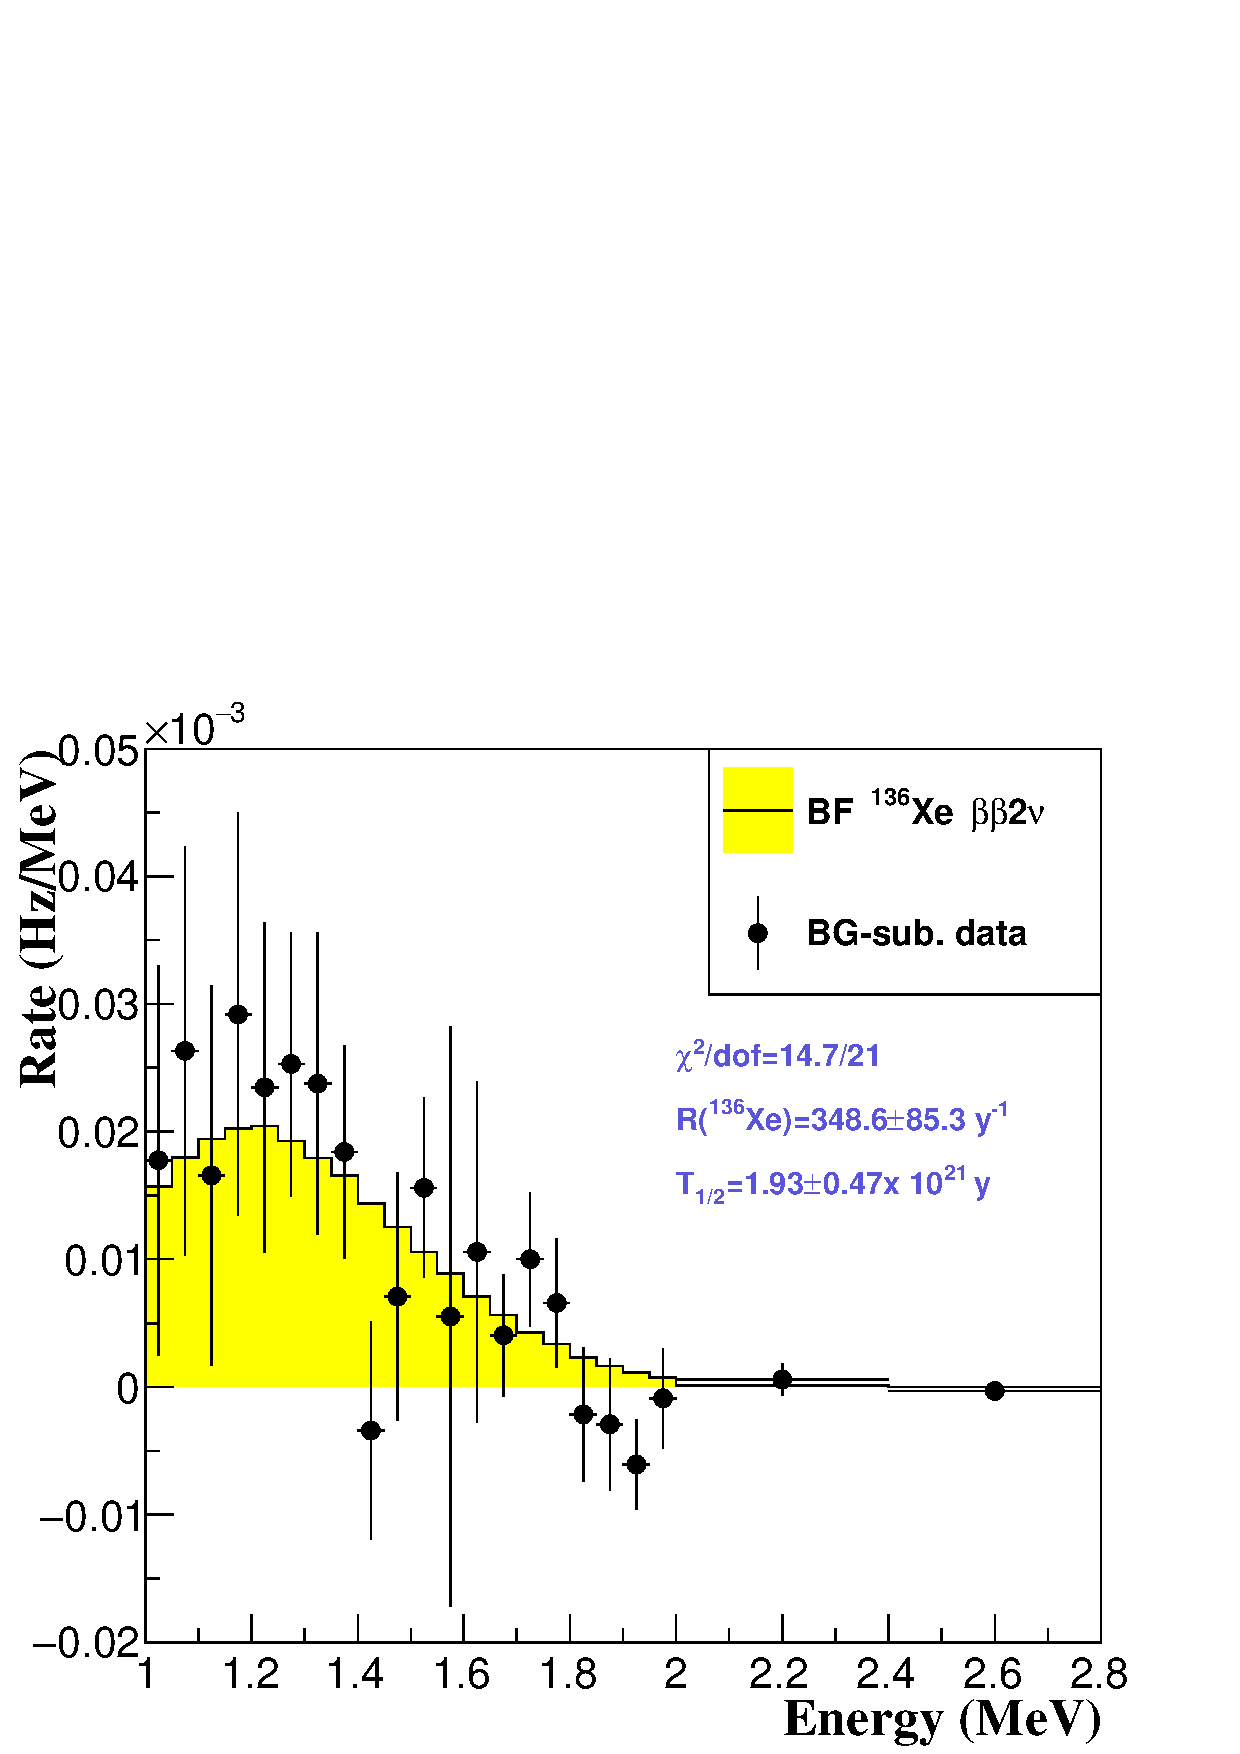
\includegraphics[width=0.31\textwidth]{img2/BGSubFit.jpg}
    \caption{Main NEXT-White results. Left: energy resolution at the 2.6 MeV \Tl{208} photo-peak (from \cite{Renner:2019pfe}). Middle: signal efficiency versus background rejection (from \cite{NEXT:2021pjq}). Right: Background-subtracted \bbtnu ~fit (from  \cite{nextcollaboration2021measurement}).} 
    \label{fig:newresults}
  \end{center}
\end{figure}



\subsection{The \Next\ apparatus}
\label{sec.next100}

\begin{figure}[htbp!]
\centering
\includegraphics[width=0.9\textwidth]{img2/NEXT-100-description.jpg}
%\includegraphics[width=0.9 \textwidth]{img/next-100.png}
\caption{\small Scheme of the \NEXT\ detector.}
\label{fig.next-100}
\end{figure}

\subsubsection{The detector}

The \Next\ detector is an asymmetric \HPXeEL\ TPC shown schematically in figure \ref{fig.next-100}.  The fiducial region is a cylinder of \NextTpcDiameter\ diameter and \NextTpcLength\ length, (\NextFiducialVolume\ fiducial volume) holding a mass of \NextFiducialMass\ of xenon gas enriched at \XeEnrichment\ in \XE, and operating at \NextPressure.  An energy plane ({\bf EP}),
made of PMTs, provides a measurement of the energy integrating the full signal (\stwo) and records the primary scintillation light (\sone) which triggers the start-of-event (\tz). A tracking plane ({\bf TP}) provides a 2D image of the tracks propagating in the detector, which is then turned into a 3D image when combined with the measurement of the drift time.  

%\indent

The TPC consists of a field cage, a cathode held at high voltage via high-voltage feedthroughs ({\bf HVFT}), and two electroluminescent meshes for the signal amplification.
The field cage is designed to be a scalable solution for a larger system (i.e, for \NHD).  The design is based on affixing copper rings to High Density Polyethylene ({\bf HDPE}) staves that run the length of the drift and buffer regions.  
A resistor chain along the field cage copper rings maintains a uniform electric field. Segmented light reflector panels made of polytetrafluoroethylene ({\bf PTFE}),  inserted into vented grooves in the HDPE staves provide enhanced light collection, and the full field cage is wrapped in a thin polyethylene insulating sheet to avoid electrical breakdowns between the field cage rings and the outer copper shielding.
The cathode, the anode and the gate (the latter two defining the EL region) consist of three large meshes.  Each mesh will consist of three large parts; the photo-etched mesh that is trapped and tensioned by a two-part frame. 

%\indent

The EP is made of 60 Hamamatsu R11410-10 photomultiplier tubes located behind the TPC cathode, with a coverage of approximately 30\%. This represents a compromise between the need to collect as much light as possible for a robust measurement of the energy and t$_0$, while minimising cost and technical complexity. However, the tradeoff is a relatively high contribution to the radioactive budget. The R11410-10 is a 3-in PMT especially developed for low-background operation, equipped with a synthetic silica window and a photocathode made of low temperature bialkali with quantum efficiency above 30\% for the emission wavelengths of xenon and TPB.
The R11410-10 cannot be run above 6 atmospheres. To overcome this limitation, the PMTs are housed in a vacuum region behind 5 mm thick sapphire windows. %(\fig\ \ref{fig.EP}). 
The PMTs are optically coupled to the windows using an optical gel with a refractive index intermediate between those of fused silica and sapphire. Tetraphenyl-butadiene ({\bf TPB}) is evaporatively coated on the external faces of the windows. 
The PMT cables route through the conduits and the central manifold to a feedthrough in the pressure vessel nozzle.  

%\indent

The TP consists of 56 boards with 64 SiPMs each for a total of 3584 sensors. With a 15.55 mm pitch, the TP overcovers the active drift volume, allowing to detect events near the PTFE walls that will be important for fiducialisation of events.
The TP is separated 15 mm from the anode grid. This distance, larger than in the NEXT-White detector, is driven by mechanical constraints. In this case, the use of thicker (6 mm) PTFE masks helps in recovering the necessary light for a correct reconstruction of the events’ topology. These masks will act as collimators, providing a narrow Point Spread Function (PSF). As SiPMs, the \Next\ TP will use the model S13372-1350TE from Hamamatsu, with 1.3x1.3 mm$^2$ active surface area. Compared to \New\ SiPMs, \Next\ SiPMs will thus detect up to 60\% more photons.
Further improvements with respect to \NEW\ include the reduction of kapton mass and glue in the front face of the boards, which will substantially reduce the radioactive budget. This is accomplished by using a single layer of kapton.

\subsubsection{Electronics and DAQ}

The TP readout is based on the high-performing and reliable \NEW\ electronics and interconnections \cite{Rodriguez:2015a}, with some mechanical modifications required to efficiently double the number of readout channels,. Signals from the SiPMs are passively fed to readout electronics placed 4-to-5 m from the detector vessel. This readout concept nearly hits a practical limit in NEXT-100: the number of wires across the vessel cannot be further scaled up without raising reliability concerns. This is the reason why \NHD\  requires a new solution that implies installing readout and multiplexing ASICs inside the vessel (see section \ref{sec.hd}). %The new readout concept for \NHD\ is described in section \ref{ASIC} and requires a 3-year R\&D program, which has already been planned and scheduled.

%\indent

The PMT readout electronics is the same  used in \NEW\ and is described in \cite{Alvarez:2019a}. Scaling up from 12 to 60 PMTs is accomplished by simple replication of 8-channel front-end modules and 12-channel digitisers. A decade of experience designing and operating PMT bases, amplifiers and digitisers have led to a sound and reliable design. %The grounded-cathode PMT connection requires AC coupling and thus a baseline restoration circuit. We have opted for a digital baseline restoration algorithm running on an FPGA, based on the inverse function of a high-pass filter, whose coefficients are tuned for each channel to ensure the best possible performance.

%\indent

Data acquisition (DAQ) and trigger systems for NEXT-100 are also based (with small modifications) on those from \NEW\, which have successfully and reliably operated for several years. Reference \cite{Esteve:2021a} describes the DAQ partitions and architecture, the double-buffer and double-processor readout to avoid detector dead time, and the configurable trigger algorithms. The advantage of the current modular DAQ and event detection system is that it has been dimensioned from the beginning to cope with the increased number of sensors in NEXT-100. Due to the modularity of the electronics and the software framework (CERN ALICE's DATE), the DAQ hardware and online system can be easily scaled.

\subsubsection{Lead Castle and Muon Veto}

In order to shield  \Next\ against external radiogenic backgrounds (\ie, gammas emanating from the laboratory walls), the detector will be operated inside a ``lead castle'', which has already been used for NEXT-White data taking. Furthermore, the internal cosmogenic backgrounds induced by muon interactions in the lead and detector materials will be mitigated by a muon-veto covering the castle surfaces, as shown in \fig\ \ref{fig.muonveto}.  Without this system, the projected background index in \Next\ would be $\sim1.2\times10^{-3}$ counts/keV/kg/yr rather than our target value of $\sim5\times10^{-4}$ counts/keV/kg/yr.   

\begin{figure}[htbp!]
\centering
\includegraphics[width=0.5\textwidth]{img2/MuonVeto_1.JPG}
%\includegraphics[width=0.4\textwidth]{img2/MuonVeto_2.JPG}
\caption{\small Scheme of the muon veto mounted on the lead castle}
\label{fig.muonveto}
\end{figure}

The muon veto will be funded by LSC, as it is considered an infrastructure of the laboratory, like the lead castle. Its construction and commissioning with the rest of the detector will be a collaboration between IFIC and LSC. The system will be made of individual modules arranged in two different layers in orthogonal directions, so the X and Y coordinates of a crossing muon can be disentangled. A total of 14 modules (with sizes between 3116$\times$2622 mm and 1124$\times$ 2622 mm) cover the external walls of the lead castle. Each one of the modules consists of a row of mechanically-joined 20 cm wide scintillator strips  (USMS-03 by UNIPLAST Inc.), placed side by side in a protective aluminum casing providing the necessary mechanical stability. Two wavelength shifting (WLS) fibers (Kuraray Y11(200)M, 1 mm diameter) are glued into two grooves in the long edges of each strip with a polysiloxane compound. Hamamatsu S12825-050P [9] silicon photomultipliers (SiPMs) are used to collect the scintillation light from the opposite side of each fiber. The SiPMs signals are sent to a commercial front-end electronics board with 32 channels (CAEN A1702), mounted at the readout end of the module, where  they are processed for storage.

\subsubsection{Status of the detector and data taking program}

\begin{figure}[!htb]
\centering
\includegraphics[width=0.8\textwidth]{img2/collage_ICS.jpg}
\caption{\small a) The NEXT-100 apparatus; b) a detail showing the inner copper shield ({\bf ICS}) inside the pressure vessel; c) detail of the gas inlet pipes through the EP; d) a detail showing the integration of the detector. ICS comes first, then field cage is slid in, then the end-caps carrying the heavy copper supports for the tracking plane and energy plane are moved in.} 
\label{fig.n100e}
\end{figure} 


All \Next\ subsystems are currently completed or in late stage of construction, with the exception of the muon veto that will be built during 2022. At the time of writing this proposal, the pressure vessel ({\bf PV}) is being installed in the refurbished lead castle (adapted to \Next\ after completing the operation of \NEW). The gas system has also been upgraded and tested. The inner copper shield  ({\bf ICS}) is being machined and will be installed in the next few months inside the PV. All the electronics is ready and tested. The three major subsystems, EP, TP and the TPC will be installed inside the vessel from March to May, 2022 (figure \ref{fig.n100e}). The detector is scheduled to start operations in June. We foresee six months for the initial commissioning and calibration ---the muon veto will be commissioned during this period---, followed by 12 months taking data with depleted xenon (background measurement) once the muon veto is installed, before the start of the run with enriched xenon. 
%The physics run will take three years (2023 to 2025). 
%During 2025, \Next\ data taking will proceed in parallel with the assembly of the \NHD\ detector and the setup of the infrastructures (\NHD\  will operate in a different area than \Next\ thus making possible the operation of the later while the former is being assembled). 

%Our project plan foresee up to one year contingency for the start-of-operations of \NHD.  \Next\  will continue operations until the new detector is ready for commissioning.  

\subsubsection{Sensitivity of \Next}

The projected background in the ROI for \Next\ is \SI{7}{\ev\per\tonne\per\yr}, with the leading background sources being the PMTs and the substrates of the SiPMs~\cite{Martin-Albo:2015rhw}.  This translates in less than one background event per year of operation, allowing the apparatus to reach 
a sensitivity of \SI{1E26}{\yr} with an exposure of \SI{500}{\kg\yr}. 

%\indent

Our current plan includes a physics run that will extend at least two of the three years of this research project. During this period we will also carry the R\&D needed for the construction of the the \NHD\ detector and its infrastructures (see next section). We foresee that the time needed to construct, integrate and commission the \NHD\ detector and infrastructures will be 2-3 years after the R\&D is completed. During all this time we plan to operate \Next\ (notice that the infrastructures for \NHD\ are different and will be located in an adjacent location at the LSC). Thus, it appears feasible to reach our original target exposure and sensitivity, which will be competitive with the best current experiments in the World. 

On the other hand, given the null results obtained 
by current-generation experiments, it is clear that all main technologies need to scale up to detector masses in the ton range as soon as possible. This is certainly the strategy of leading experiments such as LEGEND, CUPID and nEXO and is also NEXT strategy. However, simply increasing the target mass by an oder of magnitude is not enough to reach the target sensitivity of \NHD\ (\SI{1E27}{\yr}), which also requires to reduce the background to \SI{1}{\ev\per\tonne\per\yr} or less (see section \ref{sec.hd}). While \NHD\ is being designed to achieve such background reduction, the operation of \Next\ is also essential to demonstrate that our background model is accurate, and also to identify possible unexpected background sources which can be corrected for \NHD. Further goals of \Next\ are to optimise detector performance, in particular the energy resolution and the background rejection capabilities of the topological signature. We also aim to refine the technique, demonstrated in our recent \bbtnu\ analysis with \NEW\ \cite{nextcollaboration2021measurement} of measuring directly the backgrounds from the data themselves, thus minimising the background model dependence of the Monte Carlo.  





\subsection{The \NHD\ detector}
\label{sec.hd}

\begin{figure}[htbp!]
\centering
    \includegraphics[width=0.42\linewidth]{img2/cut_detector.jpg}
    \includegraphics[width=0.30\textwidth]{img2/BFDSiPM.jpg}
    \includegraphics[width=0.26\textwidth]{img2/FiberPanel.jpg}
    %\includegraphics[width=0.42\linewidth]{img/Half_5.png}
     \caption{\small Left: image of the \NHD\ detector in its vertical orientation. Middle: conceptual drawing of the BFD, showing the copper ring that cools the reaout SiPMs (option 1 for BFD readout, see text). 
     Right: conceptual drawing of  a fibre panel, in this case, connected to a PMT (option 2 for BD readout).}
     \label{fig.NHD}
\end{figure}

%\begin{figure}
%  \begin{center}
%    %\includegraphics[width=0.31\textwidth]{img/Fiber13D.png}
%    \includegraphics[width=0.31\textwidth]{img2/Fiber23D.jpg}
%    \includegraphics[width=0.25\textwidth]{img2/FiberPanel.jpg}
%    \caption{Conceptual design of the BFD (left), and of a fibre panel (right).} 
%    \label{fig.BFD}
%  \end{center}
%\end{figure}

 The HPXe technology benefits from the economy of scale inherent to homogeneous experiments in which the \bbonu\ source and the detector are the same. The necessary factor of 10 increase in fiducial mass is obtained by increasing the detector linear dimensions (parallel and perpendicular to the TPC drift direction) by slightly more than a factor of 2 compared to \NEXT. At the same time, the background rate (after cuts) must be kept in the ``quasi-zero'' regime of less than one event per year in the ROI. This requires a detector with improved radiopurity at the ton-scale. This is achieved by the combination of: {\bf i)} a reduced background budget, achieved, in particular, by eliminating the leading source of background (the PMTs of the EP, which is replaced by a low-background system, the barrel fibre detector, {\bf BFD}) and further reduce other background sources (thinner kapton boards, titanium frames for the grids and ultra-low radioactivity resistors);  {\bf ii)} improvement of the energy resolution from 1\% to 0.5--0.7\% FWHM at \Qbb, possible thanks to the better  performance of BFD which collects more light than \Next\ EP and is less affected by geometrical corrections; and {\bf iii)} improvement of the rejection power of the topological signature, by reducing the diffusion through the use of low-diffusion Xe-He mixtures and increase the density of the SiPMs coverage with respect to that in \NEW\ and \Next\ ( Dense Silicon Planes, {\bf DSP}). The resulting apparatus will have ``higher definition'' of the signal, w.r.t. previous NEXT apparatus, thus the label HD (``high definition''). 
 
 %\indent
 
The \NHD\ concept is schematically rendered in the left panel of figure \ref{fig.NHD}. %shows a conceptual rendering of the \NHD\ detector.
The major change in the design with respect to the current apparatus is the transformation to a symmetric device featuring two twin back-to-back TPCs, each  with its own EL region and connected by a central cathode. In a symmetric detector, one doubles the active region for the same cathode voltage compared to its asymmetric counterpart.  Based on geometrical considerations the required high voltage for \NHD\ will be only $\sim$ 30\% larger than that needed for NEXT-100. A symmetric detector with 2$\times$\XHDL\ drift and \XHDD\ diameter will be able to hold \XHDM\ at 15 bar. Another relevant modification with respect to NEXT-100 is the vertical detector orientation, chosen in order to simplify the assembly of the different parts of the system, in particular the heavy (about \XHDS) inner copper shield. 

%\indent

The second major change ---dictated by both the symmetric detector design and the need to reduce the background budget--- is the substitution of the energy plane (made of PMTs viewing the active volume) by an alternate energy measurement solution.  An attractive solution is a barrel detector made of wavelength-shifting optical fibres. The fibres, coated with TPB shift first the impinging VUV photons to violet photons (with an average wavelength circa \SI{420}{\nm}). Those photons are absorbed by the fibres which re-emit green light (circa  \SI{530}{\nm}). Green photons propagating by total internal reflection inside the double-clad fibres reach the fibres ends, which are grouped in bundles and read out by either PMTs or SiPMs. Our Monte Carlo studies show that the light collection of this BFD is at least 50\% larger than that of a conventional NEXT energy plane. This, together with the expected soft geometrical corrections (which, to first order, should follow a smooth radial dependence) would imply a corresponding improvement in the detector energy resolution. The BFD will also measure \sone, providing the start-of-the-event.  The middle and right panels of figure \ref{fig.NHD} show conceptual drawings. 

%\indent


The BFD will be made of \BFDNP$\times$2 panels of optical fibres. Each panel has \BFDNFPP\ fibres, which are read out by \BFDNSIPMPP\ SiPMs
of size \BFDNSIPM\ (main option) or by a PMT (alternative option). The advantage of SiPMs are their large photo-detection efficiency (near 50\% for the greens wavelengths that propagate in the fibres) and the simplicity of mechanics. The main disadvantage is the large dark current, which must be reduced by several orders of magnitude in order to detect the \sone\ of the low-energy calibration sources (\Kr{83}). This can be done by connecting the SiPMs to a copper ring which is kept at temperatures around -80 C, enough to reduce the dark current by three orders of magnitude. Conversely, the dark current of the PMTs is negligible, but the mechanics is more complex, and they are more radioactive (although they will be shielded from the main volume). Deciding between these two options will be one of the
deliverables of our proposed R\&D. 


%\indent

\begin{figure}[htbp!]
  \begin{center}
      \includegraphics[width=0.91\textwidth]{img2/tracks.jpg}
    \caption{Impact on track reconstruction of reduced diffusion and fine grain tracking planes. The left panel shows the signature of the two electrons emitted in a \bb\ decay, when reconstructed with a dense silicon plane. Notice the separation between the two ``blobs'', each one defining the end-point of one electron. The middle panel shows the same reconstruction when using a low diffusion mixture with 15\% helium. The right panel shows the final double electron, reconstructed with our sophisticated deconvolution technique (see \cite{NEXT:2020jmz}).} 
    \label{fig.DSP}
  \end{center}
\end{figure}

%\indent

Last but not least, the possibility to reduce diffusion and thus improve the rejection power of the topological signature calls for a fine granularity tracking system. Dense SiPM planes, will allow for a better measurement of the track trajectories. This  is illustrated in figure  \ref{fig.DSP}. 
Notice that the reconstruction benefits from three elements: {\bf i,} fine-grain pixelisation provided by the DSPs;  {\bf ii,} reduced diffusion through the use of  helium-xenon mixtures, and {\bf iii,} sophisticated deconvolution software developed by NEXT \cite{NEXT:2020jmz}.  As a result, the two blobs characterising the two electrons emitted in a \bb\ decay are clearly resolved most of the times, allowing an enhanced background suppression. 

%\indent

The number of channels in each DSP plane scales quadratically with the pitch. Monte Carlo simulations indicate that the minimum practical pitch is of the order of 
\DSPMNP. In this case one has \DSPMNPC\ channels and \DSPMNPB\ boards per DSP. This is to be compared with the pitch used in \NEW\ (\DSPMXP), 
which results in \DSPMXPC\ channels and \DSPMXPB\ boards per DSP plane. Finding the best compromise between pitch (cost) and performance is another of the main goals of the proposed R\&D.

%\indent

On the other hand, the large number of channels in the DSPs (even for the largest pitch considered) make unrealistic to place the front-end electronics ({\bf FEE}) outside the PV, as has been done for both \NEW\ and \Next. Thus, the new detector requires the development of in-vessel FEE. The UPV group, which has designed the FEE for the previous NEXT detectors, has expertise in the design of ASICs. We have already a design for such ASICs (described in the section of objectives for the UPV), and a program to complete prototypes and a final design in three years. In addition, new DAQ modules, which will upgrade the $\sim$10 years old DAQ modules used by \NEW\ and \Next\ will be developed by UPV. 

%\indent

Finally, the shielding of \NHD\ will be different from that of \Next. The need to suppress drastically cosmogenic backgrounds at the LSC depth (which requires a very effective veto against muon-induced neutrons and energetic gamma-rays) leads to replacing the lead structure (``lead castle'') and the muon veto used by \Next\ by an instrumented water tank ({\bf WT}), which provides a more efficient muon veto and avoid the muon-spallation background induced in the lead. In addition, the detector will have (like \NEW\ and \Next) an inner copper shield to protect the TPC volume from backgrounds emanating from the vessel. The WT is considered an infrastructure and will be built by the LSC. 


%%%%%%%%%%%%%%%%%%%%%%%%%%%%%%%%%%%%%%%%%%%%%%%%%%%%%%%%%%%%
\subsubsection{Sensitivity of \NHD}
\label{sec:BackgroundsAtTheTonneScale}
%%%

The sensitivity of \NHD\ has been extensively discussed in a recent publication \cite{NEXT:2020amj}. Here we summarise the main results. 
Our background model and event selection algorithms, described below, have been checked against the data collected by \NEW\ \cite{Novella:2019cne} and will be further validated to higher precision with the data acquired  by \Next. 

%\indent

{\bf $\bullet$~ Backgrounds of radiogenic origin}

%\indent
High-energy gamma radiation from long-lived radioactive contaminants present in detector materials and surroundings is an important background in NEXT. Particularly troublesome are two of the gamma-ray lines emitted following the decays of \Tl{208} and \Bi{214}, part of the thorium and uranium series, respectively. The gamma-ray line from \Tl{208} (2614.5~keV, 99.75\% intensity \cite{nudat}) is well above $\Qbb=\SI{2457.8}{\kilo\eV}$, the $Q$ value of \Xe{136}, but single-electron tracks from its photopeak can lose energy via bremsstrahlung and fall in the region of interest. Likewise, gammas that interact via successive Compton scatters in proximity may be reconstructed in some cases as a single track with energy close to \Qbb. The gamma-ray line from \Bi{214} (2447.7~keV, 1.55\% intensity \cite{nudat}) lies just below \Qbb, and thus its photopeak can overlap with the \bbonu\ peak due to the finite energy resolution of the detector.

%\indent

Gamma radiation emanating from laboratory walls and external support structures is unlikely to reach the inner detector through the water shielding (3~m of water attenuate this gamma flux by more than 6 orders of magnitude). For this reason, we focus on sources close to the active volume of the detector, particularly those with large mass, such as the inner copper shield. These backgrounds can be mitigated and understood by careful radio assay of all materials used in the construction of the detector. The NEXT Collaboration has undertaken extensive campaigns for the characterisation of all materials used for the \NEW\ and NEXT-100 detectors \cite{Alvarez:2012as, Cebrian:2017jzb}, primarily employing gamma-ray spectroscopy with high-purity germanium detectors and inductively coupled plasma mass spectrometry. An even more extensive and stringent campaign will be even more important for the material selection of \NHD, under the coordination of the LSC.  


%%%%%%%%%%
%\begin{table}[tb]
%\centering
%\begin{tabular}{l l l c c c}
%\toprule
%Material & Detector system & Method & \multicolumn{2}{c}{Activity ($\mathrm{\mu Bq / kg}$)} & Reference \\
%         &                 &        & \Th{232} & \U{238} & \\
%\midrule
%Copper & Inner shield   & ICPMS            & $1.22\pm0.04$   & $1.28\pm0.09$ & \cite{NEXT:2020amj} \\
%PTFE   & TPC field cage & NAA              & $0.103\pm0.012$ & $<5$          & \cite{Abgrall:2016cct} \\
%Kapton & Readout planes & ICPMS            & $81\pm15$       & $110\pm50$    & \cite{Arnquist:2019fkc} \\
%\bottomrule 
%\end{tabular}
%\caption{Specific activities of \Th{232} and \U{238} (parents of \Tl{208} and \Bi{214}, respectively) assumed in the background model of NEXT-HD for the most relevant materials used in the detector.}
%\label{tab:RadioactivityMaterials}
%\end{table}
%%%%%%%%%%

%\indent

The material that dominates the budget is copper, given the large mass (nearly 40~tons) used for the inner shield. 
%Our best activity measurement (C11000 copper supplied by Lugand Aciers, radio assayed at PNNL using ICPMS) is comparable to values reported elsewhere \cite{Kharusi:2018eqi}. 
After copper, PTFE and Kapton, two synthetic polymers, are the main contributors to the radioactivity budget of \NHD. PTFE (about \SI{500}{kg}) represents a significant fraction of the mass of the TPC field cage. Backgrounds from the pressure vessel as well as any additional infrastructure outside the detector are efficiently mitigated by the inner copper shielding. They are estimated to contribute at or below the 5\% level to the full radioactive budget. 
%Here, we use activity measurements reported in the literature \cite{Abgrall:2016cct}. In the case of Kapton, used as substrate for the SiPM support boards (each one is \SI{8.4}{g} and covers \SI{121}{cm^2}), we use recently-published measurements \cite{Arnquist:2019fkc}. 


%This number is informed by experience from \NEW\ and NEXT-100, where present upper limits sit at approximately 5--10\% of the total activity budget \cite{Martin-Albo:2015rhw, Novella:2019cne}. Any additional external sources can be effectively mitigated by increasing the thickness of inner copper shielding without significant detriment to the total activity.

%\indent

Radon is another potential source of radioactive background, since it can diffuse from detector materials or the gas system and enter the active region. Only two radon isotopes, \Rn{220} and \Rn{222}, from the thorium and uranium series, respectively, are found in significant amounts. Their production rates are similar, but the longer half-life of the latter (3.8~days versus the 56~seconds of \Rn{220} \cite{nudat}) makes it much more likely to become a background. Radon-222 undergoes two alpha decays to produce \Bi{214}, and previous NEXT measurements show that these positively-charged daughters usually plate out onto the cathode \cite{Novella:2018ewv}. The subsequent \Bi{214} decays on the cathode are rejected with high efficiency (through fiducial cuts) by the detection of the emitted beta electrons and coincident decays of \Po{214}. Rejection efficiency should only increase in a symmetric design, since the cathode would be surrounded by fully instrumented volumes. For the present study, we consider the internal radon backgrounds at a similar rate as that of the present generation of NEXT detectors~\cite{Novella:2018ewv}, a conservative assumption, given the improvements in radiopurity expected in \NHD. Additional contributions from airborne radon backgrounds from outside the vessel are expected to be negligible due to the surrounding water.

%%%%%%%%%%%%%%%%%%%%%%%%%%%%%%%%%%%%%%%%%%%%%%%%%%%%%%%%%%%%
%\indent

{\bf $\bullet$~ Backgrounds of cosmogenic origin}
\label{sec:muons}

%%%
Cosmogenic backgrounds in NEXT derive from neutron capture on detector materials, especially on copper isotopes and \Xe{136}. The main source of neutrons that induce these potential backgrounds are atmospheric muons with energies up to a few TeV that reach the laboratory through the rock overburden. 
%Neutron capture produces two types of potential background: prompt activity from gamma radiation post-capture, and the creation of long-lived nuclei with decays that can result in events at energies close to \Qbb. The former is dominated in NEXT by contributions from the capture of neutrons on the two main copper isotopes via the reactions $^{63,65}\text{Cu}(n, \gamma)^{64,66}\text{Cu}$ \cite{nudat}, but there are also contributions from captures on plastics and on the steel pressure vessel. The cascade photons from all of these various reactions have energies up to tens of MeV. As the interactions in the gas occur within a few ms of the passage of a muon, these events can be rejected without significant reduction to detector live-time, introducing a veto of \SI{2}{\milli\second} after the tagging of a muon in the water tank or the TPC. Any remaining events contribute at a negligible level.

%\indent

%Non-prompt backgrounds derive from the production of long-lived isotopes that later decay with $Q$ values above \Qbb. 
The dominant contribution to this background comes from the beta-emitter \Xe{137}, produced by single-neutron capture on \Xe{136}. Xenon-137 decays with a half-life of \SI{3.8}{minutes} and a $Q$ value of \SI{4.17}{\mega\eV} \cite{nudat}. This background is difficult to veto by time coincidence with a detected muon due to the excessive dead-time that it would generate. 

%%%%%%%%%%
\begin{figure}
\centering
\includegraphics[width=0.55\textwidth]{img2/BlobComparison.jpg}
\includegraphics[width=0.40\textwidth]{img2/sensitivity_nexthd_lsc.jpg}
\caption{Left: blob energies of signal and background events. The blobs are defined such that \emph{blob 1} always has higher energy. Right: sensitivity of \NHD.}
\label{fig:blobs}
\end{figure}
%%%%%%%%%
%%%%%%%%%%%%%%%%%%%%%%%%%%%%%%%%%%%%%%%%%%%%%%%%%%%%%%%%%%%%
%\indent

{\bf $\bullet$~ Signal efficiency and background rejection}
\label{sec:SimulationAndAnalysis}

%\indent
We evaluated the signal efficiency and background rejection of \NHD\ following the methodology described in \cite{Martin-Albo:2015rhw, NEXT:2020amj}. Signal events in NEXT have a distinctive energy-deposition pattern: a continuous track with large energy deposits (or \emph{blobs}) at both ends. Background events, in contrast, are generated mostly by single electrons, thus having only one end-of-track blob. The separation between signal and background events is illustrated in the left panel of figure~\ref{fig:blobs}, which shows the blob energy distributions for all signal and background events generated for the study. The figure of merit indicates a threshold of \SI{400}{\kilo\eV} as the optimal for the lower blob energy.

%\indent

The main components of the radioactive budget before and after selection cuts are presented in figure \ref{fig:ActivityComp}. The contribution of the cosmogenically-induced \Xe{137} is 2.5 times as large as the radiogenic background at the depth of LSC (2500~m.w.e.). Nevertheless, the cosmogenic background could be mitigated with the addition of \He{3} to the xenon as a means to moderate and capture neutrons, reducing the number of activations in the detector volume. A reduction in the number \Xe{137} of over 1 order of magnitude could be achieved with as little as 0.1\% by mass of \He{3} doping \cite{rogers2020mitigation}. The possibility to procure \He{3} for the NEXT experiment is being explored by the US groups in the collaboration. 

%%%%%%%%%%
\begin{figure}[tb]
\centering
\includegraphics[width=0.90\textwidth]{img2/RadioactiveBudget2.jpg}
\caption{Left: Total background activity before cuts for the dominant sources in the \NHD\ radioactivity budget. Right: Activity remaining after selection cuts.}
\label{fig:ActivityComp}
\end{figure}
%%%%%%%%%%

%%%%%%%%%%
%\begin{table}
%\centering
%\begin{tabular}{lccS[table-format=2.2e-1]}
%\toprule
%Det.\ system & \multicolumn{2}{c}{Acceptance [$10^{-8}$]} & {Background index} \\
% & \Tl{208} & \Bi{214} & {[$\mathrm{ton^{-1}~yr^{-1}~ROI^{-1}}$]} \\
%\midrule
%Field cage        & 6.80(90) & 6.30(80) &  4.25e-3 \\ \addlinespace
%Readout planes    & 6.80(90) & 7.80(80) &  1.36e-3 \\ \addlinespace
%Inner shielding   & 4.50(70) & 1.20(70) & 37.23e-3 \\ \addlinespace
%Radon (cathode)   & ---      & 0.10(10) &  2.72e-3 \\ 
%\bottomrule
%\end{tabular}
%\caption{Acceptance factor (i.e., the probability of accepting a background event as signal) and resulting background indexes per unit of mass of \Xe{136} for the natural-radioactivity background sources considered in the background model of \NHD.}
%\label{tab:radiogenics}
%\end{table}
%%%%%%%%%%

%%%%%%%%%%
%\begin{table}
%\centering
%\begin{tabular}{lcS[table-format=2.2e-1]}
%\toprule
%Source gas & Acceptance  & {Background index} \\
% & [$10^{-5}$] & {[$\mathrm{ton^{-1}~yr^{-1}~ROI^{-1}}$]} \\
%\midrule
%Pure xenon & \multirow{2}{*}{5.68(17)} &  113.49e-3\\ \addlinespace
%0.1\% \He{3} doping &  & 11.78e-3 \\ 
%\bottomrule
%\end{tabular}
%\caption{Acceptance factor for the \Xe{137} background and resultant contribution to the background index of NEXT-HD at the LSC.}
%\label{tab:cosmogenics}
%\end{table}
%%%%%%%%%%


%%%%%%%%%%%%%%%%%%%%%%%%%%%%%%%%%%%%%%%%%%%%%%%%%%%%%%%%%%%%
%\indent

{\bf $\bullet$~ Projected sensitivity to neutrinoless double-beta decay}
\label{sec:sensitivity}
%%%

%\indent
%%%%%%%%%%
%\begin{table}[tb]
%\centering
%\begin{tabular}{ll}
%\toprule
%Source mass (\Xe{136}) & \SI{1109}{\kg} \\
%Signal efficiency      & \num{24.6}{\%} \\
%Background rate        & \SI{0.010}{\keV^{-1}.\tonne^{-1}.\year^{-1}} \\
%                       &
%\SI{0.168}{ROI^{-1}.\tonne^{-1}.\year^{-1}} \\
%Energy resolution      & \num{0.5}{\%}~FWHM at \SI{2458}{\keV}\\
%\midrule
%$\overline{T}_{1/2}$ (\SI{5}{\tonne.\year})  & \SI{1.2E27}{\year} at 90\% CL  \\
%$\overline{T}_{1/2}$ (\SI{10}{\tonne.\year}) & \SI{2.0E27}{\year} at 90\% CL  \\
%\bottomrule
%\end{tabular}
%\caption{Key parameters for the calculation of the sensitivity of \NHD\ and resulting mean lower limit (at 90\% CL) on the \bbonu-decay half-life for 5 and \SI{10}{\tonne.\year} of exposure.}
%\label{tab:Next1tParameters}
%\end{table}
%%%%%%%%%%
%Table~\ref{tab:Next1tParameters} lists the experimental parameters that enter the calculation of the sensitivity of \NHD. 
%The total background index is calculated by adding the radiogenic and cosmogenic contributions (see Tables~\ref{tab:radiogenics} and \ref{tab:cosmogenics}) estimated in section~\ref{sec:SimulationAndAnalysis}. 
The sensitivity projected for \NHD\ can be seen in the right panel of  figure~\ref{fig:blobs}. In less than 5~years of operation, \NHD\ could reach a half-life sensitivity of \SI{1.2E27}{\year} (90\% CL), improving current limits by more than one order of magnitude. 

%%%%%%%%%%
%\begin{figure}
%\centering
%\includegraphics[width=0.85\textwidth]{img/sensitivity_nexthd_lsc.pdf}
%\caption{Projected sensitivity (90\% CL) to the \Xe{136} \bbonu\ half-life for a NEXT ton-scale experiment located at LSC. \label{fig:Sensitivity}}
%\end{figure}

%%%%%%%%%%

\section{\small  OBJETIVOS, METODOLOGÍA Y PLAN DE TRABAJO - OBJECTIVES, METHODOLOGY AND WORK PLAN}


%\subsection{General objectives and match to the National Programme for research aimed at the Challenges of Society}

\subsection*{General objectives}

The four main objectives of this proposal are:
\begin{enumerate}
\item {\bf The scientific exploitation of the \Next\ detector}. This includes the integration \& commissioning of the apparatus and the operation through the physics run, initially foreseen for three years. The deliverables are: {\bf i,} physics results produced by \Next\ which include a precise measurement of the \bbtnu\ mode, a search for \bbonu\ events in \XE\ decays, with a sensitivity competitive with other leading experiments worldwide, and other searches, such as the search for \bbonu\ events in \XEX\ decays; {\bf ii,} a precise measurement of the detector performance, including energy resolution, topological signal and radioactive budget. This deliverable is of uppermost importance for the second objective. 
\item {\bf The construction, commissioning and operation of \HDEMO}, as a platform to test the solutions to be implemented in \NHD.  
\item {\bf Selection and screening of materials for \NHD}. As discussed in the previous section, the radioactive budget of \NHD\ must be carefully controlled. This requires an extensive campaign of material selection and screening which will include the copper for the shielding and TPC, the steel (or titanium) for the vessel and grids, the PTFE for the light tube, fibres, SiPM circuit boards, resistors, etc. 
\item {\bf Preparation of the infrastructures for \NHD}. The operation of \NHD\ will require substantial new infrastructures at the LSC, including: {\bf i,} a new water tank to veto muons, {\bf ii,} an upgrade of the gas system, {\bf iii,} the preparation of the inner copper shield of the detector. 
\end{enumerate}

\indent

The scientific exploitation of the \Next\ detector (objective {\bf 1}) will be responsibility of DIPC, IFIC,  USC and UPV. The four institutions will cooperate in the operation of the detector itself (which requires day-by-day monitoring, slow-controls and shifts). DIPC will be in charge of run coordination, USC will lead the calibration of the detector and IFIC will provide analysis tools. UPV will be in charge of slow-controls and monitoring. All the institutions will collaborate in the physics analysis.  

\indent

The \HDEMO\ detector (objective {\bf 2}) will be built and operating through the collaboration of DIPC, IFIC, USC and UPV (with the help of international partners). 
During the first two years of the project IFIC will build the pBFD (together with WIS and BGU from Israel), UPV will build the pDSP (in collaboration with Harvard) and a prototype of the front-end electronics and DAQ, DIPC will build the pTPC, the pressure vessel and the gas system, and USC will prepare the reconstruction software as well as the Monte Carlo simulation of the detector. 

The material selection and screening campaign for \NHD\ (objective {\bf 3})  will be coordinated by LSC, in close collaboration with the NEXT groups. 

The preparation of the infrastructures for \NHD (objective {\bf 4})  will be lead by LSC, with the participation of the NEXT institutes, in particular DIPC and IFIC, who will be in charge of integrating the \NHD\ detector with the shielding and gas system infrastructures.

Detailed schedules are presented in the section on Methodology.  
  
\subsection{Objectives of the \sDIPC\ subproject}
\label{sec.obj.dipc}

DIPC takes three major roles in this project: {\bf i:} coordinates the integration, commissioning and operation of \Next\ (in collaboration with IFIC); 
{\bf ii:} hosts and participates in the construction, commissioning and operation of the \HDEMO\ prototype, and 
{\bf iii:} co-coordinates \NHD\ integration (in collaboration with IFIC and LSC). 

   
\subsubsection*{Integration, coordination and operation of \Next}

\indent

%\begin{figure}[!htb]
%\centering
%\includegraphics[width=0.7\textwidth]{img2/Next100Collage.jpg}
%\caption{\small a) The NEXT-100 apparatus; b) a detail showing the ICS inside the pressure vessel; c) a detail showing the integration of the detector. ICS comes first, then field cage is slid in, then the end-caps carrying the heavy copper supports for the tracking plane and energy plane are moved in.} 
%\label{fig.n100e}
%\end{figure} 
%

Integration of \Next\ components will proceed during the first half of 2022. The integration task, in which all the subsystems (EP, TP, TPC and ICS) are assembled inside the \Next\ PV and the full detector is placed inside the lead castle (figure \ref{fig.n100e}), will be coordinated by the DIPC, and involves directly the Technical Coordinator, two senior engineers who server as integration managers ({\bf IMs}) and the {\bf GLIMOS}, who is an expert in safety and links with the LSC personnel. The TC, the GLIMOS and one of the IMs are personnel from DIPC, while the second IM is from IFIC. 

The commissioning and operation of the system will occur during the second half of 2022 and involves the Run Coordinator ({\bf RC}), who has the following crucial functions: 


\indent

\begin{itemize}[noitemsep,topsep=0pt,parsep=0pt,partopsep=0pt]
\item {\bf Monitor the day-by-day operation of the detector}, ensuring that safety protocols are met and operation parameters are respected. This includes the status of the gas system, the high voltages, and the sensors's voltage. All those systems are followed by slow-controls which can react automatically to emergencies such as over pressure ---that situation would trigger an automatic gas recovery---, voltage excursions ---which would result in an automatic voltage shutdown--- etc. Nevertheless, the status of the detector must be assessed every day, to guarantee safe and stable operations in the long term and correct any potential problem, such as leaks, broken channels etc. DIPC coordinated the operation of \NEW, acquiring invaluable experience during the 5 years-long run. 
 
\item {\bf Monitor physics parameters},  in particular the electron lifetime, who has a major impact in the energy resolution. Again, the experience of \NEW\ will be important here. The initial electron lifetime of the former detector was \SI{100}{\micro\second}, to be compared with the lifetime in the physics runs, in excess of 
\SI{10}{\milli\second}, \eg, an improvement of two orders of magnitude, which was achieved as we developed the know-how on the technology. 

\item {\bf Organise the shifts}, both in-person (scientists and engineers present at the LSC) and remote (scientists following on-line the detector evolution). The RC organises weekly run-coordination meetings where all the aspects of detector's operation are discussed. 
\end{itemize}

\indent

\subsubsection*{\HDEMO\ prototype}

\indent

The \HDEMO\ prototype will be hosted at the DIPC, which provides a full equipped laboratory, including a state-of-the-art gas system.  During the first two years of the project, DIPC will design the pressure vessel (PV) and explore the options of building it with low-radioactivity steel alloy (as previous NEXT apparatus), or with titanium, which could reduce the PV mass and radioactive budget. The TPC, including field cage, light tube, anode and cathode grids and HVFT will also be built.  During the first half of the third year, the two new systems, pBFD (built by IFIC) and pDSP (built by UPV) will be installed. Operation of the detector will be crucial to test and validate the new systems in \NHD. 

\subsubsection*{Coordination of the \NHD\ integration}

The interface between the \NHD\ detector itself and the surrounding infrastructures is a crucial element that must be addressed for the ton-scale apparatus as early as possible. Unlike previous NEXT incarnations, \NHD\ will be immersed in water, inside a large tank. Access to the detector implies emptying (and then refilling) the tank at considerable economic cost and implying a long shutdown, typically of three to six  months. It is therefore imperative that all interfaces are as robust as possible. Here, the term ``interface'' refers to:

\begin{itemize}[noitemsep,topsep=0pt,parsep=0pt,partopsep=0pt]
\item {\bf High Voltage feedthroughs}:  With two drift lengths of \XHDL\ the central cathode will be at a voltage of \XHDHV, while the gates creating the electroluminescence in the anodes will be at \XHDELHV. The voltages will be supplied through insulated cables that connect to the high voltage feedthroughs (HVT). \item {\bf Signals and high voltage for the sensors}:  The digitised signals produced by the in-vessel, front-end electronics that reads the DSPs SiPMs and the BFD fibres must be transported, through insulated pipes to the DAQ located outside the water tank. The sensors require (moderate) high voltage to operate, which requires additional ports.
\item {\bf Gas}:The flow of gas must also be channeled through pipes from the external gas system to the detector, penetrating the water tank. detector must be placed inside the water tank and connected to the gas system. 
\end{itemize}

\indent

The {\em definition} of all the above infrastructures requires the specification of each port in the \NHD\ high pressure vessel, as well as the specification of the ports in the water tank, the definition of the specs of the cables and pipes and substantial testing. 
\indent

A second major task is the integration of the inner copper shield (ICS). The ICS will be made of ultra-pure copper, with a mass of \XHDS. LSC will select, screen and purchase the copper, and will also be in charge of machining it, following the scheme that has been implemented in \Next. The final product will be bars and disks, with a thickness of \XHDCS, each of them weighting at least one ton (considerably more in the case of the disks). The integration of the ICS inside the \NHD\ pressure vessel requires also a precise design, as well as a well defined protocol for installation. 

\indent

In all the above tasks, DIPC and IFIC will serve as co-coordinator, drawing on the experience acquired in previous apparatus by the two senior mechanical engineers, that will be in charge (S. C\'arcel from IFIC and J. Torrent from DIPC). 

\subsubsection*{Personnel in the Working Plan}
The working plan for \sDIPC\ involves 8 FTEs (J.J. G\'omez-Cadenas, F. Monrabal, P. Ferrario, F. L\'opez-Guejo, A. N\'u\~nez J. Torrent, J.L. L\'opez, E. Oblak) and three Ph.D. students (Pablo Herrero, Leire Larizgoitia and Beatriz Romeo). The responsibilities on the project of the existing personnel are:


\begin{itemize}[noitemsep,topsep=0pt,parsep=0pt,partopsep=0pt]
\item J.J. G\'omez-Cadenas is co-spokesperson and executive spokesperson of the NEXT collaboration. He is in charge of the overall coordination of the project. 
\item F. Monrabal is the technical coordinator of the collaboration. He coordinates the integration and operation of \Next, as well as the \HDEMO\ project.
\item  F. L\'opez-Guejo is the project manager  for both \Next and \NHD.
\item P. Ferrario is an expert in simulation and analysis and will be involved in the reconstruction software and Monte Carlo development for \Next, \HDEMO and \NHD, in collaboration with USC. 
\item J. Torrent is a senior mechanical engineer. He is one of the Integration Managers of \Next\ (the other is S. C\'arcel, from IFIC) and will co-coordinate the integration of \NHD. 
\item A. N\'u\~nez is a senior engineer. She is acting at the GLIMOS  for \Next. 
\item E. Oblak is a  mechanical engineer. She  will work in the design of \NHD\ vessel and the design of \HDEMO.  
\item J.L. L\'opez is a technician, that will assist in the construction and operation of \HDEMO. 
\end{itemize}

We request for this project two post-docs. Post-doc 1 (PD1) will work as a Run Coordinator (supervised by F. Monrabal) and will work in \Next\ data analysis, in particular in the topological reconstruction, under the supervision of P. Ferrario. Post-doc 2 (PD2) will work in the \HDEMO\ detector, under the supervision of J.J. G\'omez-Cadenas and F. Monrabal. He or she will work during the first two years in the design and construction of the
\HDEMO\ TPC, grids and HVFT, and during year three in the commissioning and operation of \NHD. 

The project is extremely suited for students, given the large training potential of our project, which includes detector operation, data analysis, Monte Carlo simulation, and the opportunity to contribute to the construction and operation of a cutting edge HPXe, the \HDEMO\ demonstrator. In this project we apply for one FPI position. 

\subsection{Objectives of the \sIFIC\ subproject}
\label{sec.obj.dipc}
\subsubsection*{Integration and operation of \Next}

\indent

IFIC contributes to the integration of \Next\ with a senior engineer (S. C\'arcel) who co-coordinates the integration of the system with J. Torrent (DIPC). In addition, IFIC is responsible for the maintenance of the \Next\ gas system. 

\indent

IFIC will contribute to the operation of the \Next\ detector, providing shifters, and will play a major role in the development of analysis tools and in the
physics analysis themselves. In particular, IFIC will lead the \bbtnu\ measurement. 


\subsubsection*{\HDEMO\ prototype}

\indent

IFIC will conduct the R\&D towards the construction of the BFD detector and will produce the pBFD prototype. 
 

\subsubsection*{Coordination of the \NHD\ integration}

IFIC will collaborate with DIPC and LSC in the definition of the \NHD\ interfaces and integration of \NHD. 



\subsubsection*{Personnel in the Working Plan}
The working plan for \sIFIC\ involves XXX FTEs (Michel, Justo, Pau, Sara...) and YYY Ph.D. students (Alberto...). The responsibilities on the project of the existing personnel are:


\begin{itemize}[noitemsep,topsep=0pt,parsep=0pt,partopsep=0pt]
\item M. Sorel and P. Novella are physics co-conveners. 
\end{itemize}

We request for this project XX post-docs. 

The project is extremely suited for students, given the large training potential of our project, which includes detector operation, data analysis, Monte Carlo simulation, and the opportunity to contribute to the construction and operation of a cutting edge HPXe, the \HDEMO\ demonstrator. In this project we apply for one FPI position. 

\subsection{Objectives of the \sUSC\ subproject}
\label{sec.obj.dipc}
\subsubsection*{Operation of \Next}

\indent

USC will contribute to the operation of the \Next\ detector, providing shifters, and will play a major role in the development of software tools (reconstruction software, Monte Carlo simulation). USC will also lead the calibration of the detector. 


\subsubsection*{\HDEMO\ prototype}

\indent

USC will be in charge of developing the software for \HDEMO, including reconstruction and simulation of the system. 
 



\subsubsection*{Personnel in the Working Plan}
The working plan for \sIFIC\ involves XXX FTEs (JA, Josh) and YYY Ph.D. students (Gonzalo...). The responsibilities on the project of the existing personnel are:


\begin{itemize}[noitemsep,topsep=0pt,parsep=0pt,partopsep=0pt]
\item J.A. Hernando is the software coordinator of NEXT.  
\end{itemize}

We request for this project 1 post-doc. 

The project is extremely suited for students, given the large training potential of our project, which includes detector operation, data analysis, Monte Carlo simulation, and the opportunity to contribute to the construction and operation of a cutting edge HPXe, the \HDEMO\ demonstrator. In this project we apply for one FPI position. 

\subsection{Objectives of the \sUPV\ subproject}
\label{sec.obj.dipc}
\subsubsection*{Operation of \Next}

\indent

UPV will contribute to the operation of the \Next\ detector, providing the maintenance of all the front end electronics modules, the DAQ modules, the online cluster and the slow controls. 


\subsubsection*{\HDEMO\ prototype}

\indent

UPV will be in charge of developing the front-end electronics and DAQ for \HDEMO.
 
\subsubsection*{FEE and DAQ for \NHD}

\indent

UPV will be in charge of developing the front-end electronics and DAQ for \NHD (Asics, etc). 
 



\subsubsection*{Personnel in the Working Plan}
The working plan for \sUPV\ involves XXX FTEs (Vicente, Raul, Curro...). The responsibilities on the project of the existing personnel are:


\begin{itemize}[noitemsep,topsep=0pt,parsep=0pt,partopsep=0pt]
\item V. Herrero is in charge of the FEE... 
\end{itemize}

We request for this project XXX

\subsection{Objectives of the \sUPV\ subproject}
\label{sec.obj.dipc}

\subsubsection*{Coordination of screening measurements for \NHD}

\indent

LSC will coordinate the screening measurements for \NHD. 
 
\subsubsection*{Infrastructures for \NHD}

\indent

LSC will build the WT and ISC. LSC will purchase de xenon.   
 

\subsubsection*{Personnel in the Working Plan}
The working plan for \sLSC\ involves XXX FTEs (Carlos...). The responsibilities on the project of the existing personnel are:


\begin{itemize}[noitemsep,topsep=0pt,parsep=0pt,partopsep=0pt]
\item Carlos... 
\end{itemize}

We request for this project one physicist and one engineer. 

\subsection{Methodology}



The specific objectives of all the subprojects are integrated in the NEXT Project Management Plan (PMP). The PMP has been used to organise the construction and operation of \NEW, and is currently managing the integration, commissioning and operation of \Next. 
The PMP has been essential for the construction of both apparatus. In particular, the \Next\  project drew from the experience gained while building \NEW, resulting in optimised procedures for the construction of the detector and the development of the electronics and software. The PMP for \NHD\ currently under development draws on the experience acquired building \Next\ and is an essential tool to manage the project.  
\indent

%\begin{figure}
%  \begin{center}
%    \includegraphics[width=0.91\textwidth]{img/pmp-n100.png}
%    \caption{A sketch of the NEXT PMP showing the main projects and \Next\ subprojects} 
%    \label{fig.pmps}
%  \end{center}
%\end{figure}

%\begin{figure}
%  \begin{center}
%    \includegraphics[width=1.0\textwidth]{img/pmp-nhd.png}
%    \caption{A sketch of the NEXT PMP showing the main projects and the main \NHD subprojects prior to construction. } 
%    \label{fig.pmp}
%  \end{center}
%\end{figure}

%The five groups involved in this proposal collaborate in the projects defined above:
%
%\begin{itemize}[noitemsep,topsep=0pt,parsep=0pt,partopsep=0pt]
%\item {\bf NEXT-100}: integration of the final detector is being led by DIPC and IFIC, with participation of the international collaboration. USC is in charge of the software development and maintenance. UPV is in charge of the electronics, DAQ and slow controls. IFIC, DIPC and USC collaborate in the physics (IFIC leads the development of physics tools and USC the calibration procedures). All the groups participate in the data taking and daily operations of the apparatus. 
%\item {\bf NEXT-HD R\&D}: the R\&D effort will focus in the \HDEMO\ apparatus. IFIC will lead the construction of the BFD prototype, UPV of the DSPs and associated electronics, DIPC will be in charge of the infrastructures (gas system and shielding), pressure vessel and TPC. The three groups will collaborate in the integration. USC will prepare the software, simulation and calibration procedures. 
%\item {\bf NEXT-HD R\&D}: The DSPs of the \NHD\ detector will have near 200,000 channels. This makes imperative using integrated front-end electronics. UPV will be leading the effort of developing an ASICs, for the DSPs, drawing on their experience with \Next\ front-end electronics. In addition they will develop an upgraded version of the existing DAQ. 
%\item {\bf NEXT software}:  NEXT software includes the offline reconstruction, online monitoring, automatic calibration software, Monte Carlo simulation and analysis tools. All the software components are fully operative for \NEW\ and \Next\ apparatus and will be upgraded for \NHD\ under the leadership of USC.  
%\end{itemize}
 

\indent

The PMP is under the direct supervision of NEXT executive spokesperson and coordinator of this proposal (G\'omez-Cadenas). He is assisted by a project manager (PM) who combines an extensive technical preparation with experience in logistics. DIPC has hired a dedicated person for this task (F. L\'opez-Guejo), who is currently serving as \Next\ PM. To ensure that the software for \NHD\ is developed also under controlled protocols, the collaboration has appointed a software coordinator (SC, J.A. Hernando, PI of the \sUSC\ project). 

\indent
 
The PMP defines and follows the progress of a set of Working Packages (WP), monitoring deliverables and deadlines and keeps track of invested resources including personnel. It also identifies potential show-stoppers and synergies (as well as possible conflicts) between the different projects and optimises the sharing of resources. 

\indent

The methodology of each WP includes: a) the definition of the associated tasks; b) the identification of the resources needed; c) the temporal organisation of the tasks; d) the definition of milestones and the deliverables associated to them; e) the relations with other WP. Each WP has a leader, who reports directly to the project managers. The progress of each WP is reviewed on a bi-weekly basis. Milestones and potential showstoppers are discussed, and the tracking charts updated if needed.

Coordination and monitoring of the various WP activities is ensured via a number of regular meetings within the NEXT Collaboration, run on a weekly or bi-weekly basis: These are the  {\em hardware} meeting, chaired by the technical coordinator, {\em software} meeting, chaired by software coordinator, and {\em analysis} meeting, chaired by the physics analysis conveners (PC, Michel Sorel and P. Novella from IFIC). The {\em project} meeting, chaired by the co-spokesperson (assisted by the PM), runs usually on a monthly basis, and involves the technical coordinator, software convener and physics conveners as well as the integration coordinator, the run coordinator and the leaders of the working packages. 

\indent

While it is not possible to capture all the details of the PMP\footnote{Detailed GANTT charts can be found in the NEXT web page, XXXX} in this document, we present a brief summary of the main projects in tables \ref{tab:schedule_n100}, \ref{tab:pmp_elec_nhd}, \ref{tab:pmp_hdemo}, \ref{tab:pmp_nhd_infra} and
\ref{tab:pmp_nhd}. Table  \ref{tab:schedule_n100} shows the schedule for the integration, commissioning and operation of \Next; 
table \ref{tab:pmp_elec_nhd} shows the schedule for the development of the electronics, table  \ref{tab:pmp_elec_nhd} details the R\&D for the \HDEMO\ prototype, and table \ref{tab:pmp_nhd_infra} shows the schedule for the development of the infrastructures for \NHD. All those activities will develop during the period
2022-2025, relevant for this project. For completeness, in table \ref{tab:pmp_nhd}, we show the foreseen schedule for the construction, integration and operation of \NHD.


\begin{table}[h!]
\begin{center}
\begin{tabular}{| l | c | c | c | c |}
\hline
Tasks & 2022 & 2023 & 2024 & 2025 \\
\hline
Integration  & Q1-Q2& -&-& -  \\
%\hline
Commissioning  & Q3-Q4 &-&- & -  \\
%\hline
Depleted xenon run &- & Q1-Q4 &- &-   \\
%\hline
Enriched xenon run  & -& - & Q1-Q4&  Q1-Q4 \\
\hline
\end{tabular}
\caption{Timetable for the integration, commissioning and operation of \Next.}
\label{tab:schedule_n100}
\end{center}
\end{table} 


\begin{table}[h!]
\begin{center}
\begin{tabular}{| l | c | c | c | c |}
\hline
Tasks & 2022 & 2023 & 2024 & 2025 \\
\hline
Prototype FEE  & Q1-Q2& -&-& -  \\
%\hline
Prototype DAQ  & Q1-Q2 &-&- & -  \\
%\hline
Production FEE \& DAQ for \HDEMO &- & Q1-Q4 &- &-   \\
%\hline
Final design FEE \& DAQ for \NHD  & -& - & Q1-Q4&  - \\
Production FEE \& DAQ for \NHD  & -& - & &  Q1-Q4 \\
\hline
\end{tabular}
\caption{Timetable for the development of \NHD\ electronics.}
\label{tab:pmp_elec_nhd}
\end{center}
\end{table} 

\begin{table}[h!]
\begin{center}
\begin{tabular}{| l | c | c | c | c |}
\hline
Tasks & 2022 & 2023 & 2024 & 2025 \\
\hline
R\&D pFBD  & Q1-Q2& -&-& -  \\
%\hline
R\&D pDSP  & Q1-Q2 &-&- & -  \\
R\&D pTPC, Vessel, HVFT \& Grids  & Q1-Q2 &-&- & -  \\
%\hline
\HDEMO\ construction  &- & Q1-Q4 &- &-   \\
%\hline
\HDEMO\ integration  & -& - & Q1-Q2&  - \\
\HDEMO\ commissioning  & -& - & Q3-Q4&  - \\
\HDEMO\ run  & -& - & -&  Q1-Q4 \\
\hline
\end{tabular}
\caption{Timetable for the development of the \HDEMO\ prototype.}
\label{tab:pmp_hdemo}
\end{center}
\end{table} 


\begin{table}[h!]
\begin{center}
\begin{tabular}{| l | c | c | c | c |}
\hline
Tasks & 2022 & 2023 & 2024 & 2025 \\
\hline
Selection \& screening of copper for ICS  & Q1-Q2& -&-& -  \\
%\hline
Design of Water Tank  & Q1-Q2 &-&- & -  \\
R\&D pTPC, Vessel, HVFD \& Grids  & Q1-Q2 &-&- & -  \\
%\hline
Procurement of copper  &- & Q1-Q4 &- &-   \\
%\hline
Machining of copper  & -& - & Q1-Q2&  - \\
Conditioning of \HDEMO\ experimental area  & -& - & Q1-Q2&  - \\
Construction of Water Tank  & -& - & Q3-Q4&  - \\
Upgrade of gas system  & -& - & -&  Q1-Q2 \\
\hline
\end{tabular}
\caption{Timetable for the construction of \NHD\ infrastructures.}
\label{tab:pmp_nhd_infra}
\end{center}
\end{table} 

\begin{table}[h!]
\begin{center}
\begin{tabular}{| l | c | c | c | c |}
\hline
Tasks & 2026 & 2027 & 2028 & 2029 \\
\hline
Construction of BFD, DSP and TPC  & Q1-Q4& -&-& -  \\
%\hline
Construction of PV, HVFT and Grids  & Q1-Q4 &-&- & -  \\
Production of electronics modules  & Q1-Q2 &-&- & -  \\
%\hline
Integration with ICS and WT  &- & Q1-Q2 &- &-   \\
Commissioning  &- & Q3-Q4 &- &-   \\
%\hline
Physics run  & -& - & Q1-Q4& Q1-Q4 \\
\hline
\end{tabular}
\caption{Timetable for the construction of \NHD.}
\label{tab:pmp_nhd}
\end{center}
\end{table} 







\subsection{Budget request}

%This coordinated project requires funding for the continuation of a 10 year-long effort in the NEXT-program.
%
%The infrastructures already existing for the experiment as well as the \NEW\ detector have been co-funded by the CONSOLIDER-INGENIO project CUP (2009-2014), which provided 5 million \euro, and an AdG/ERC project granted to G\'omez-Cadenas (2014-2019), which provide 2.8 million \euro. The LSC has contributed to many of the infrastructures and also owns the enriched xenon that will be used by \Next\, whose estimated cost today exceeds 2 million \euro\ (only three groups in the world own large amounts of enriched xenon, KamLAND-Zen experiment, EXO experiment and the LSC). 
%  
% The infrastructures already available at the LSC include: the working
% platform and seismic table (LSC infrastructure); the lead castle (LSC
% infrastructure); a radon abatement system (LSC infrastructure) that
% injects radon-free air into the volume surrounding \Next, among other experiments; a clean tent (LSC infrastructure) surrounding all the experiment; a sophisticated gas system (AdG/ERC as well as contributions from Portugal and USA); a large emergency evacuation tank (AdG/ERC); electrical, vacuum and pressure equipment such as UPSs, pumps and gaskets (AdG/ERC); the \NEW\ detector (AdG/ERC funds); the \Next\ pressure vessel (purchased using CUP funds); a large fraction of the detector PMTs were also purchased using CUP funds.
 
 This coordinated project requires funds for:
 \begin{itemize}[noitemsep,topsep=0pt,parsep=0pt,partopsep=0pt]
\item Scientific exploitation of the \Next\ detector (including costs of operation at the LSC). 
%\item Computing for \Next\ at the LSC.
\item Maintenance of the \Next\ infrastructures (mainly the gas system). 
\item Radioactive sources for calibration. 
\item Construction of the \HDEMO\ prototype. 
%\item Preparation of the infrastructures for \NHD.
\item Essential personnel. 
\item Travel other than the LSC (NEXT workshops and attendance to international conferences).
\item Others (small equipment, maintenance of local laboratories, etc.). 
\end{itemize}

\subsubsection{Costs of operations at the LSC}
\label{sec:operationcost}
The costs of \Next\ operations at the LSC, will be distributed among the four groups participating in the project. The costs are estimated after five years of operation of \New\ and are, therefore, very accurate. They include rental of an apartment plus appliances (1,000 \euro/month, which is much cheaper than lodging personnel in hotels), travel and allowances for shifters and engineers.  The costs of the apartment are assigned to DIPC. The cost of travel and allowances is distributed among the four groups taking into account the personnel traveling to LSC in each group. The cost of travel is computed assuming that the group in charge of the shifts (rotates every week) rents a car ---rental cars are the only practical way to arrive to Canfranc, and to access the laboratory---. The cost of the cheapest rental car is estimated as 400 \euro/week. Concerning maintenance, we keep it to a minimum (50 \euro\ per day and person), which covers meals while at LSC. Therefore, we estimate 750 \euro\ per week and shifter. Two shifters are needed for regular operations, 40 weeks per year. The total number of person-shifts is 80, which adds up to 60,000 \euro/year (180,000 \euro\ for 3 years).

The shifts are run by the whole collaboration, but the burden of shifts at LSC is taken by the Spanish and Portuguese groups, while the remote shifts are mostly run by US and Israel groups. After the experience running \NEW\, we have found that the four groups participating in this project run 40\% of the shifts at the LSC, the rest of the Spanish and Portuguese groups run 40\% and the US and Israel groups run the remaining 20\% and most of the remote shifts. This results in a total of 
72,000 \euro\ for shifts. Given the relative size of the groups, we request 20,000 \euro\ for DIPC and IFIC and 16,000 \euro\ for USC and UPV.

\subsubsection{Costs of maintenance of \Next\ infrastructures}

The costs of maintenance, specified in table \ref{tab.main}, are dominated by the gas system and are accurately estimated after the long operation of \NEW. Maintenance is a must for the proper performance and safety of the experiment. Since IFIC is in charge of the maintenance of the gas system, this cost is assigned to the \sIFIC\ subproject.

\begin{table}[h!]
\begin{center}
\begin{tabular}{|l|r|r|r|}
\hline
Part & 	Cost (\euro/year)	& Years	& Subtotal (\euro) \\
\hline
Pump maintenance	& 1000	& 3	& 3000\\
Compressor              & 4,000 &	3	& 12,000 \\ 
Repair of equipment	& 5,000 &	3	&15,000 \\
Cleaning products and operations	& 2,000 &	3 & 6,000 \\
Gas supply (Ar, He, N$_2$)  & 5,500 & 	3 &	16,500 \\
Electronics spares & 4,000   & 3 & 12,000\\
Miscellanea (gaskets, valves, spares)	& 6,000 &	3 & 18,000 \\
Tooling	& 8,000 & 3 & 24,000 \\
\hline
{\bf Total} & & & {\bf 106,500}\\
\hline
\end{tabular}  
\caption{Maintenance of \Next\ (\sIFIC).}
\label{tab.main}
\end{center}
\end{table} 


\subsubsection{Costs of radioactive sources for calibration}

Another fixed cost is that of radioactive sources. Table \ref{tab.calib} details the cost of the conventional sources (\Kr{83} and \Th{228}). Since USC is in charge of calibration, this cost is assigned to the \sUSC\ subproject.

\begin{table}[h!]
\begin{center}
\begin{tabular}{|l|r|r|r|}
\hline
Part & Cost (\euro/unit) & Units & Subtotal (\euro) \\
\hline  
Kr-83 &	3,000 &	3 & 9,000 \\
Th-228 &	12,000 & 1 & 12,000 \\
\hline
{\bf Total }   &  & &  {\bf 21,000} \\
\hline
\end{tabular}  
\caption{Radioactive sources for calibration (\sUSC).}
\label{tab.calib}
\end{center}
\end{table}

\subsection{Other travel, small equipment and lab maintenance}
\label{sec:othercosts}

NEXT holds two Collaboration Meetings (CMs) per year (December and May) at the LSC. The dates are adjusted to the meeting of the LSC Scientific Committee, which takes 2 days, and the meeting takes 2 days right before the LSC-SC meeting. We request funding for attendance of the members of the project to the CMs, at a very adjusted budget of 400 \euro/week and person.

The NEXT Collaboration is regularly invited to present results in international conferences. We request funds for two conferences during the three years for senior members and post-docs, and one conference plus one school during the three years for students.

Finally, each group requests a modest amount of funding for small equipment and maintenance of laboratories at home institutions (10,000 \euro\ per group and year). 

%\subsubsection{Costs of computing at the LSC}

\subsubsection{DIPC}

DIPC brings considerable resources to the project. The total number of FTEs working in the project is 9. DIPC has provided a large laboratory for \HDEMO\ and the funds to equip it with a state of the art gas system (already purchased) which includes: the gas loop (50 k\euro), compressor (140 k€),
vacuum system (15k\euro), leak detector (12 k\euro), High Voltage sources (20 k\euro), and lab equipment, including scope, picoamperimeter, tools, etc 
(about 30 k\euro). In total, DIPC has invested more than 300 k\euro in the \HDEMO\ lab. 
 
DIPC requests:

\begin{itemize}[noitemsep,topsep=0pt,parsep=0pt,partopsep=0pt]
\item {\bf Costs of personnel}: PD1 (run coordinator) and PD2 (\HDEMO):  50,000 \euro\ per year and person, for a total of 300,000 \euro\ \item {\bf Operation of \Next\ at the LSC}. Cost of the apartment at Canfranc: 12,000 \euro\ per year for a total of 36,000 \euro\ and cost of shifts 20,000 \euro\ (see sec.\ref{sec:operationcost}) 
%\item Operation of \Next\ at the LSC. Shifts: 20,000 \euro.
\item {\bf Cost of the \HDEMO\ pressure vessel}: 100,000 \euro.
\item {\bf Cost of the \HDEMO\ TPC} (items are detailed in the Web formulary):  35,000 \euro.
\item {\bf Consumables for the \HDEMO\ laboratory}: 10,000 \euro.
\item {\bf Xenon for \HDEMO\ prototype}: 4 kg, at a cost of  12,000 \euro\ per kg (48,000 \euro\ total). 
\item {\bf Travel} other than the LSC (NEXT workshops and attendance to international conferences): 48,000 \euro\ for the whole team. 
\item {\bf Small equipment}: 10,000 \euro.
\end{itemize}

The total requested direct cost is 607,000 \euro. 

\subsubsection{IFIC}

IFIC brings to the project 5 FTEs and an equipped laboratory for the R\&D of NEXT-HD, where the pBFD detector will be developed and operated. The IFIC laboratory has hosted the previous NEXT prototypes and offers the infrastructures for the proposed R\&D line (clean room, gas system, vacuum vessels, dark boxes, vacuum monochromator, light sources and oscilloscopes, among others), with an approximate investment in excess of 350,000 \euro. 

The cost estimate for the \sIFIC subproject is listed below:
\begin{itemize}[noitemsep,topsep=0pt,parsep=0pt,partopsep=0pt]
    \item {\bf Personnel}: 47,000 \euro\ per year for senior electronic engineer E1 (\Next\ maintenance, muon veto FEE and DAQ and NEXT-HD R\&D), 40,000 \euro\ for postdoc PD3 (scientific exploitation of \Next\ including muon veto), for a total of 261,000 \euro  
    \item {\bf NEXT-100 maintenance}: 106,500 \euro\ (see Tab.\ref{tab.main})
    \item {\bf NEXT-100 operation (shifts)}: 20,000 \euro\ (see Sec.\ref{sec:operationcost})
    \item {\bf Consumables for the IFIC laboratory}: 10,000 \euro\ (see Sec.\ref{sec:othercosts})
    \item {\bf BFD R\&D and pBFD}: 100,0000 \euro\ in total (items are detailed in the Web formulary). 
%     divided in
%        \begin{itemize}
%            \item fibers sensors and electronics: 7,5000 \euro
%            \item optomechanic elements: 7,500 \euro
%            \item vessel for pBFD mock-up: 10,000 \euro
%            \item fibers for pBFD panels: 10,000 \euro
%            \item sensors and readout for pBFD: 10,000 \euro
%            \item mechanics and coating of pBFD: 5,000 \euro
%            \item gases (Ar, Xe, N2): 10,000 \euro
%            \item computing (hard disks, processors): 10,000 \euro
%            \item radioactive sources: 10,000 \euro
%            \item development of cold electronics for SiPMs: 13,500 \euro
%            \item general electronics: 20,000 \euro
%        \end{itemize}
    \item {\bf Attendance to Collaboration Meetings}: 19,200 \euro\ (see Sec.\ref{sec:othercosts})
    \item {\bf Conferences and schools}: 20,000 \euro\ (see Sec.\ref{sec:othercosts})
\end{itemize}

The total direct cost is 550,200 \euro.

\subsubsection{UPV}
UPV brings to the project CAD (Computer Aided Design) software licenses through Europractice foundation as long as foundry access for MPW (MultiProject Wafer) prototypes and short production series. 

The cost estimate for the ASIC development draws on estimated device areas per design iteration for a typical 180nm node process (XFAB). This includes a possible rework due to high failure risk when dealing with silicon designs (selected process offers at least two foundry windows per year). The number of dies assumes a 80\% yield. 

The cost estimate for the \sUPV subproject is listed below:
\begin{itemize}[noitemsep,topsep=0pt,parsep=0pt,partopsep=0pt]
    \item {\bf Personnel}: 47,000 \euro\ per year for a senior electronics engineer for DAQ, test boards and slow controls, and 37,000 \euro\ per year for a 
junior microelectronic engineer for silicon design. The total amounts to a total of 252,000 \euro.
\item {\bf ASIC development}: The total cost (items are detailed in the Web formulary) is 301,500 \euro.
\item {\bf DAQ development}: The total cost (items are detailed in the Web formulary) is 67,000 \euro. 
\item {\bf Travel}, including both maintenance at LSC and attendance to collaboration meetings: 29,400 \euro. 
\item {\b Conferences and schools}: 6,000 \euro.
\end{itemize}

The total direct cost is 655,900 \euro.


%\begin{itemize}[noitemsep,topsep=0pt,parsep=0pt,partopsep=0pt]
%    \item AF single channel test chip (10 mm2 - 20 units) + packaging: 17,000 €
%    \item Test Boards for test chip 1 (estimated): 3,000 €
%    \item FPGA development boards for CH prototyping (estimated): 15,000 €
%    \item AF for \HDEMO\ (20 mm2 - 80 dies) + packaging: 41,500 €
%    \item Test Boards for AF \HDEMO\ (estimated): 3,000 €
%    \item FPGA components and boards for AF and CH in \HDEMO\ 20,000 €
%    \item AF final design (40 mm2 - 100 dies) + packaging: 80,000 €
%    \item Test Boards for AF final design (estimated): 3,000 €
%    \item Extra run costs for rework: 80,000 €
%    \item FPGA components and boards for AF and CH final design 20,000 €
%    \item Europractice maintenance fees for 3 years: 9,000 €
%    \item General equipment for CAD (servers, disk storage): 10,000 €
%\end{itemize}

%The cost estimate for DAQ research and development (items are detailed in the Web formulary) is 67,000 \euro. 
%\begin{itemize}[noitemsep,topsep=0pt,parsep=0pt,partopsep=0pt]
%    \item Slow Controls - CompactRIO modules (2) + Extra hardware: 5,000 €
%    \item DAQ - Read Out (5): 20,000 €
%    \item DAQ - Chassis (1): 6,000 €
%    \item DAQ - Computing (2): 10,000 €
%    \item DAQ - Cabling: 1,000 €
%    \item DAQ - Prototyping costs: 10,000 €
%    \item Small equipment and maintenance: 15,000 €
%\end{itemize}

%The costs of personnel include a senior electronics engineer for DAQ, test boards and slow controls: (45,000 \euro\ per three year for a total of 135,000 \euro) and a 
%junior microelectronic engineer for silicon design: (45,000 \euro\ per three year for a total of 111,000 \euro).
%
%    \item Travel expenses plus diets for: 29,400 €
%    \item Conferences and Schools: 6,000
%\end{itemize}
%The total direct cost of the subproject is 641,500 €

\subsubsection{USC}
UPC brings to the project 2 FTEs and 3 Ph.D students. USC intensively use the computing resources of the ``Galician Supercomputacional Center'', CESGA. The cost for the \sUSC project is

\begin{itemize}[noitemsep,topsep=0pt,parsep=0pt,partopsep=0pt]
    \item {\bf Personnel}: a postdoc position for a technical software coordinator, 40,000 \euro\ per year, for a total of 120,000 \euro.
    \item {\bf Radioactive sources}: 21,000 \euro.
    \item {\bf Operation of NEXT-100}, shifts: 16,000 \euro.
    \item {\bf Attendance to Collaboration meetings}: 14,000 \euro.
    \item {\bf Conferences and schools}:  16,000 \euro.
    \item {\bf Computers and consumables}: 10,000 \euro.
\end{itemize}

The total direct cost is: 197,000 \euro.
\subsubsection{LSC}

LSC brings to the project 5.5 FTEs and and investment in excess of 1 M\euro (including the purchase of the \Next\ muon veto parts, and the \NHD\ infrastructures), plus the cost of the xenon. The cost for the \sLSC\ project is strictly personnel, specifically 2 senior physicist/engineer positions, for 3 years each, at a cost of 
50,000 \euro\ per year, for a total of 300,000 \euro.
 

\section{\small  IMPACTO CIENTÍFICO-TÉCNICO - SCIENTIFIC-TECHNICAL IMPACT}
\label{sec.impact}

%\subsection{Scientific and technological impact}

Establishing if the neutrino is a Majorana particle is one of the most important questions yet unanswered in particle physics. Majorana neutrinos, together with CP violation are a necessary ingredient of leptogenesis, an thus the only known way to explain the cosmic asymmetry between matter and antimatter. Majorana neutrinos are also handy to explain the smallness of neutrino masses through the see-saw mechanism. It follows that {\em demonstrating} that neutrinos are indeed their own antiparticles, would be a major scientific achievements.

The only practical way to search for Majorana neutrinos is through the study of \bbonu\ processes. Observation of a \bbonu\ decay implies necessarily that the neutrino is its own antiparticle. On the contrary, the no-observation of the process does not rule out Majorana neutrinos, given the existence of cancelations in the decay probability for very light masses. 

Neutrinoless double beta decay experiments need to deal with the fact that the lifetimes of \bbonu\ processes are known to be very long (in excess of $10^{26}$ year, and very likely at least an order of magnitude larger) and with the fact that natural radioactivity and cosmogenic backgrounds are many orders of magnitude those of the putative signal. Consequently, they face the challenge to design apparatus deploying a large mass of the target isotope, while at the same time devising experimental techniques to reduce the huge background to virtually zero. 

NEXT is one of the major experimental programs currently being developed, as evidenced in the recent APPEC report \cite{Giuliani:2019uno}. It was also one of the four experiments presented in the recent {\it North America- Europe Workshop on Future Double Beta Decay}\footnote{\url{https://agenda.infn.it/event/27143/}}. The conclusions of the workshop highlighted the high potencial of the NEXT technology, in particular due to Barium Tagging. On the other hand, the program presented in this proposal is a necessary step towards the development of a ton-scale detector able to reach the target sensitivity of the next generation of experiments
($10^{27}$ year) by extending and improving the technology developed by NEXT so far. The Barium Program R\&D, financed both in the US and in Europe (in particular through Synergy Grant "BOLD"), will be developed in parallel with the R\&D and construction of a ton-scale detector. Both programs can converge in a few years, resulting in a ton-scale detector with barium tagging, able to search for \bbonu\ events with virtually zero background, and thus capable to push the sensitivity to  $10^{28}$ year and beyond, with a very large potential for a scientific discovery.

The development of the NEXT experiment places Spain among the World leaders in a major scientific program. The development of the HPXe technology has only been possible thanks to the acquisition of the scientific know-how and the logistics to build a large scientific instrument. Last but not least, the the project has been able to involve the industrial sector at many different levels. Remarkably, the experiment ---and Spain, as host--- competes with other projects, such as LEGEND, CUPID or nEXO, which have a much longer development and can mobilise, a priori, larger resources. This is so because NEXT has managed to consolidate a full value chain, including a critical mass of national academic and industrial partners and singular facilities such as the LSC.  

This has important implications regarding the impact of the project beyond the scientific boundaries:
\begin{itemize}[noitemsep,topsep=0pt,parsep=0pt,partopsep=0pt]
\item The construction of NEXT detectors requires some national industrial partners to go beyond their own current capacities. The development of state-of-the-art technologies contributes to augment their international visibility and strengthens their showcase portfolio, helping them to diversify into markets such as those of large scientific instruments. 
\item  NEXT provides support to the aforementioned industrial partners both by sharing know-how and by collaborating with them in attracting funding. Sources of this funding can be both public competitive calls and/or private investment. Such focused investment with clear and ambitious technical targets optimises the use of funds.  
\item The successful development of NEXT will demonstrate that LSC can be a reliable long term partner, with a clear role within the global network of underground laboratories. While LSC cannot compete in size and depth with some other underground facilities ---like the LNGS, at Gran Sasso, in Italy--- it is strategically well placed within European soil, has easy horizontal access and can adapt its resources in a flexible and reliable manner. This will rise the international profile of this national singular facility and attract new relevant scientific projects in fields such as quantum technologies, biology and particle physics. 
\item On the individual scale, it is worth stressing that NEXT unusual environment provides many young scientist, engineers and technologist with rather unique work experience. The interaction with companies eases the transfer of these professionals back and forth  between the academic and industrial environments, a process which is still a major barrier form many. 
\end{itemize}

The technological output of the project deserves a detailed look on its own. A complex instrument such as the HPXe detector implements a large number of new technologies, many of them pushed to unprecedented limits of performance. While is it possible that applications of some of these technologies remains still unforeseen, in some other cases we have already identified domains of application with important economical and societal impact: 

\begin{itemize}[noitemsep,topsep=0pt,parsep=0pt,partopsep=0pt]
\item The HPXe detector integrates technology used to detect and characterise the light events taking place within the xenon contained inside the detector. This technology can be implemented in Positron Emission Tomography instruments that will use xenon (in this case in liquid form, for increased density) instead of scintillating crystals such as LYSO.  This concept is being explored by ERC Starting Grant PETALO (granted to Associate IKERBASQUE Professor P. Ferrario, one of the NEXT leading researchers) and by a Competitive Purchase (Compra P\'ublica Innovadora), launched by Generalitat Valenciana.

\item The R\&D associated to barium-tagging is opening a new inter-disciplinary field. Our approach incorporates elements of organic chemistry, atomic physics, nuclear physics, particle physics, laser-matter interactions, and photonics. It involves the technology of \HPXeEL\ chambers, ion sources, magnetic-traps, and lasers (both visible and IR). There is a clear potential to develop experimental techniques associated to our experiments that go beyond our particular needs and have wide applications. This has been acknowledged by the ERC Synergy Grant awarded to G\'omez-Cadenas, Coss\'io and Guenette. can be used for detection of other molecules, or elements such as viruses, in extremely low concentrations. 
\end{itemize}

\section{\small  IMPACTO SOCIAL Y ECONÓMICO - SOCIAL AND ECONOMIC IMPACT}
\label{sec.social}

\subsection{Dissemination of results}

%\indent
The results of the experiment will be amply advertised. NEXT is very visible in social media\footnote{Instagram: @the\_next\_experiment,
Twitter: @NEXT100Exp,
Facebook: @NextExperiment} and we are putting together, in collaboration with LSC, a science museum at ``Casa de los Abetos'', a refurbished building at Canfranc. In addition to science demonstrators (such as a cloud chamber), the museum will have a virtual tour through the underground lab and experiments, and will display outreach posters and films. A number of art works will also be displayed, as well as a section on the history of the science at Canfranc. 

%\indent

LSC and DIPC will hire jointly a person in charge of outreach and dissemination, to take care of LSC and NEXT web pages, keep the museum materials up to date and work in social media. In addition, G\'omez-Cadenas
is the science-advisor of the well known JotDown magazine, and develops an intense outreach activity which involves interviews to scientific personalities, including, recently, a Nobel Prize laureate (Kajita) and the CERN general director (Gianotti).

%\subsection{Technology transfer}
%The NEXT project has already resulted in a promising application for society, that of a TOF-PET based in liquid xenon (PETALO). Associate IKERBASQUE Professor P. Ferrario (DIPC) has been awarded an StG/ERC to develop this concept.
%



\section{\small CAPACIDAD FORMATIVA - TRAINING CAPACITY}
\label{sec.training}
\subsection{\label{subsubsec:training}Training plan}

\indent 

This coordinated project requests 4 Ph.D. fellowships (\sDIPC, \sIFIC\ \sUSC\ and \sUPV). The students will be enrolled in the Nuclear and Particle Physics doctorate programs at University of Pais Vasco, University of Valencia and University of Santiago de Compostela and Electronics Engineering doctorate programs at Universitat Politècnica de València. As part of their training, students will attend at least one international school. Students will also spend a fraction of their time in international institutions participating in NEXT: Harvard, Fermilab, Texas University, Ben Gurion University, Weizmann Institute of Science and Coimbra University.

\indent 

This coordinated project is highly multi-disciplinary, offering the students the capability of cross-training and of developing skills in a variety of areas, given the wide scope of NEXT R\&D, the sophisticated data reconstruction with algorithms suitable for medical physics, development of Deep Neural Networks for pattern recognition, and state-of-the-art instrumentation. Students in this coordinated project will rotate between different areas of work (and groups) to acquire a wide background, on hardware and software, before settling onto a specific topic.

\subsection{Supervision of Ph.D. theses and career development of former Ph.D. students}

The scientific exploitation of \Next\ offers a great opportunity for graduate students and post-docs, who typically take leading roles in important parts of the experiment. The NEXT Collaboration follows a publication model in which the main authors of the analysis are the first authors (as opposed to the general trend in the field of particle physics, which uses alphabetical order). The goal of this policy is to facilitate the visibility of graduate students and young post-docs, and to encourage them to take leading roles in the development of the experiment and the analysis of the data. Student and post-docs regularly present their results in the most relevant conferences of the field, and apply to competitive calls such as RyC and ERC. Ferrario recently obtained a StG/ERC grant for building a medical PET, PETALO.

\subsubsection*{\sDIPC\ subproject}
The COORD subproject includes three senior physicists, G\'omez-Cadenas, Ferrario and Monrabal. G\'omez-Cadenas has advised (or co-advised) a total of 15 students.  Ferrario is advising one student in PETALO (Romo). Monrabal is advising two student in NEXT (Felkai, Larizgoitia) and will co-advise one student in \Bapp-tagging R\&D (Mart\'{i}nez).

As explained in the scientific project, COORD proposes at least one additional student who will share his or her time between NEXT analysis and \Bapp-tagging R\&D. In addition, Ferrario will advise at least one student on PETALO (funded by ERC).

\subsubsection*{\sIFIC\ subproject}
M. Sorel has co-supervised two Ph.D. theses: A. Tornero ({\it ``Study of neutral pion production via neutrino-induced, charged-current interactions in the K2K SciBar detector''}, 2008), now Radio-physicist at Hospital
Universitario Dr. Negrin; and J. Catal\`a ({\it ``Measurement of neutrino induced charged current neutral pion production cross section at SciBooNE''}, 2014), now Data Scientist at Blue Trail Software. He is currently co-advising two Ph.D. students, both of them in NEXT (B. Palmeiro, A. Us\'on). P. Novella is co-supervising one Ph.D. student in NEXT (A. Us\'on) and another one in T2K (M. Antonova). J. Mart\'in-Albo has co-supervised a PhD thesis in NEXT-White (M. Nebot, {\it Calibration and background model of the NEW detector}, 2017, now Postdoctoral Research Associate at University of Edinburgh) and is currently supervising another Ph.D. student in working on the DUNE experiment (P. Amedo). L\'opez-March is co-advising one Ph.D. student in NEXT (R. Felkai). The NEXT-IFIC group is participating in EU H2020 grants focused on training ({\it ``Elusives''}, H2020-MSCA-ITN-2015) and staff exchange ({\it ``InvisiblesPlus''}, H2020-MSCA- RISE-2015-690575), to the benefit of current and prospective students in the group.

\sIFIC\ requests one Ph.D. fellowship to work on the data taking and \bb\ analysis activities in \Next\ (under the supervision of P. Novella and M. Sorel). The student will have the opportunity to contribute also to the NEXT-HD R\&D program at IFIC.


\subsubsection*{\sUPV\ subproject}
V. Herrero is co-advising one Ph.D. student (V. Alvarez) in NEXT collaboration. R. Esteve has supervised two Ph.D. theses: C.A. Marín ({\it ``PADRE pixel read-out architecture for Monolithic Active Pixel Sensor for the new ALICE Inner Tracking System in TowerJazz 180 nm technolog''}),  E.J. García ({\it ``Novel Front-end Electronics for Time Projection Chamber Detectors''}) and co-supervised one Ph.D. thesis: J.M. Monzó ({\it ``Estudio e implementación de algoritmos digitales para la mejora de la resolución temporal en sistemas de tomografía por emisión de positrones''}). F. Mora has supervised three Ph.D. theses: J.J. García-Garrigos ({\it ``Development of the Beam Position Monitors for the Diagnostics of the Test Beam Line in the CTF3 at CERN''}), C.A. Luján ({\it ``Adquisición y Procesamiento Digital de Imátenes para la Obtención de la Trayectoria de los Vectores de Posición del Camarón y la Jaiba''}), J.F. Toledo ({\it ``Study and design of the readout unit. Module for the LHCb experiment''}) and co-supervised one thesis: S. Coll ({\it ``A strategy for efficient and scalable collective communication in the quadrics network''}). F.J. Ballester has co-supervised three Ph.D. theses: M.A. Acosta ({\it ``Sistema de Alerta temprana para la predicción del nivel de peligrosidad en inundaciones pluviales repentinas''}), J.A. Canals ({\it ``Análisis y desarrollo de nuevas arquitecturas eficientes VLSI para la implementación de algoritmos basados en "Fast Search Block Matching''}), A. Mora ({\it ``Estudio de Arquitecturas VLSI de la etapa de predicción de la compensación de movimiento, para compresión de imágenes y video con Algoritmos full-search. Aplicación al estándar H.264/AVC''}). J.F. Toledo has supervised one Ph.D. thesis: J. Rodríguez ({\it ``Study and design of the front-end and readout electronics for the tracking plane in the NEXT experiment''}) 


\subsubsection*{\sUSC\ subproject}

Hernando has co-supervised two Ph.D. theses in the LHCb experiment: Mart\'{i}nez-Santos ({\it ``Study of the very rare decay $B_s\to\mu^+\mu^-$ in LHCb''}, 2010) and Cid Vidal ({\it ``Search for the rare decays $B^0_{(s)}\to\mu^+\mu^-$ and $K^0_S\to\mu^+\mu^-$ with 1~fb$^{-1}$ at LHCb''}, 2012), on one of the most important results of LHC run-I. He supevised one Ph.D. thesis in NEXT: Mart\'{i}nez-Lema ({\it ``Calibration and energy resolution of NEXT-White"}, 2018). Mart\'{i}nez-Santos was awarded the Young Experimental Physicist Prize by the European Physical Society (EPS) in 2013 and obtained in 2015 a StG/ERC grant. He is now Scientific Staff at IGFAE. Cid Vidal has been CERN fellow and is now at IGFAE with a RyC fellowship. Hernando is currently co-advising three Ph.D. students, both of them in NEXT (G. D\'{i}az, C. Hervés, M. Pérez).

\sUSC\ requests one Ph.D. fellowship.
\section{\small  CONDICIONES ESPECÍFICAS PARA LA EJECUCIÓN DE DETERMINADOS PROYECTOS – SPECIFIC CONDITIONS FOR THE EXECUTION OF CERTAIN PROJECTS}
\label{sec.specs}
None.

\section{Bibliography}
\bibliographystyle{JHEP}
%\bibliographystyle{NextRefsStyle}
\bibliography{NextRefs}

\end{document}
